\documentclass[11pt, pdf, compress, handout]{beamer}

% \usetheme{CambridgeUS}
% \usecolortheme{dolphin}
\usepackage{amsmath}
\usepackage{amssymb}
\usepackage{amsfonts}
\usepackage{algorithmicx}
\usepackage{algpseudocode}
\usepackage{hyperref}
\usepackage[utf8]{inputenc}
\usepackage{graphicx}
\graphicspath{{./figures/}}
\usepackage[english]{babel}
\usepackage{url}
\usepackage{color}
\usepackage{xcolor}

\usepackage{tcolorbox}

\definecolor{darkgreen}{RGB}{0,128,0}
 
\hypersetup{
  colorlinks,
  citecolor=darkgreen,
  linkcolor=black
}

\usepackage{natbib}

\title{Support Vector Machines}
\author{Benoit Gaüzère}


\def\dbR{{\mathrm{I\hskip-2.2pt R}}}
\def\dbN{{\mathrm{I\hskip-2.2pt N}}}
\def\esp{{\mathrm{I\hskip-1.5pt E}}}
\def\pr{{\mathrm{I\hskip-2.2pt P}}}
\def\halam{{\widehat{\lambda}}}
\def\hasig{{\widehat{\sigma}}}
\def\hae{{\widehat{\varepsilon}}}
\def\tQ{{\widehat{Q}}}

\def\tR{{\widehat{R}}}
\def\halpha{{\widehat{\alpha}}}
\def\haa{{\widehat{a}}}
\def\ha{{\widehat{a}}}
\def\he{{\widehat{\varepsilon}}}
\def\hb{{\widehat{b}}}
\def\hab{{\widehat{b}}}
\def\haE{{\widehat{E}}}
\def\hsigma{{\widehat{\sigma}}}
\def\hay{{z}}
\def\baR{{\overline{R}}}
\def\baE{{\overline{E}}}
\def\baX{{\overline{X}}}
\def\bax{{\overline{x}}}
\def\baY{{\overline{Y}}}
\def\bay{{\overline{y}}}
\def\barY{{\overline{Y}}}
\def\mx{{\overline{x}}}
\def\my{{\overline{y}}}
\def\lamMV{{\widehat{\lambda}_{MV}}}
\def\lamef{{\widehat{\lambda}_{e}}}

%\def\dbC{{\mathrm{I\hskip-5.4pt C}}}
\def\dbC{{\mathds{C}}}
\def\un{{\mathds{1}}}
\def\a{{\mathrm{a}}}
\def\b{{\mathrm{b}}}
\def\bc{{\mathrm{c}}}
\def\d{{\boldsymbol{d}}}
\def\e{{\mathrm{e}}}
\def\m{{\mathrm{m}}}
\def\n{{\mathrm{n}}}
\def\p{{\mathrm{p}}}
\def\r{{\mathrm{r}}}
\def\s{{\mathrm{s}}}
\def\u{{\mathrm{u}}}
\def\v{{\mathrm{v}}}
\def\ones{{\boldsymbol{\mathbb{1}}}}
\def\w{{\boldsymbol{w}}}
\def\x{{\mathbf{x}}}
\def\X{{\boldsymbol{X}}}
\def\y{{\boldsymbol{y}}}
\def\z{{\boldsymbol{z}}}
\def\tx{{\widetilde{x}}}
\def\bPhi{{\mathrm{\Phi}}}
\def \habeta{{\widetilde{\beta}}}
\def\Cmat{{\boldsymbol{C}}}

\def\tL{{\widetilde{L}}}
\def\tF{{\widetilde{F}}}
\def\tM{{\widetilde{M}}}
\def\tH{{\widetilde{H}}}
\def\tD{{\widetilde{D}}}
\def\tU{{\widetilde{U}}}
\def\vh{{\bar{v}^\top}}
\def\det{{\mbox{det}}}
\def\atimes{{\alert{\times}}}

\def\clO{{\mathcal{O}}}
\def\clA{{\mathcal{A}}}
\def\clB{{\mathcal{B}}}
\def\clD{{\mathcal{D}}}
\def\clL{{\mathcal{L}}}
\def\clN{{\mathcal{N}}}
\def\clH{{\mathcal{H}}}
\def\clT{{\mathcal{T}}}
\def\clY{\mathcal{Y}}
\def\fl{{\mbox{fl}}}

%\input{notation}

%%%%%%%%%%%%%%%%%%%%%%%%%%%%%%%%%%%%%%%%%%%%%%%%%%%%%%%%%%
\def\dbC{{\mathrm{I\hskip-4.7pt C}}}
\def\dbR{{\mathrm{I\hskip-2.2pt R}}}
\def\un{{\mathrm{I\hskip-5.9pt 1}}}
\def\dbN{{\mathrm{I\hskip-2.2pt N}}}
\def\esp{{\mathrm{I\hskip-1.5pt E}}}
\def\pr{{\mathrm{I\hskip-2.2pt P}}}
\def\hpr{\widehat{\mathrm{I\hskip-2.2pt P}}}
%\def\balpha{{\mathbf{\alpha}}}
\def\a{{\mathbf{a}}}
\def\b{{\mathbf{b}}}
\def\bc{{\mathbf{c}}}
%\def\d{{\mathbf{d}}}
\def\e{{\mathbf{e}}}
\def\f{{\mathbf{f}}}
\def\g{{\mathbf{g}}}
\def\h{{\mathbf{h}}}
\def\p{{\mathbf{p}}}
\def\q{{\mathbf{q}}}
\def\u{{\mathbf{u}}}
\def\v{{\mathbf{v}}}
%def\x{{\mathbf{x}}}
\def\xb{{\overline{x}}}
\def\yb{{\overline{y}}}
%\def\w{{\mathbf{w}}}
\def\haF{{\widehat{F}}}
\def\hap{{\widehat{p}}}
\def\R{\mathbb{R}}
\def\P{\mathbb{P}}
\def\E{\mathbb{E}}
\def\bX{\mathbb{X}}
\def\haF{{\widehat{F}}}
\def\haf{{\widehat{f}}}
\def\ham{{\widehat{m}}}
\def\haM{{\widehat{M}}}
\def\hamu{{\widehat{\mu}}}
\def\hasigma{{\widehat{\sigma}}}
\def\hap{{\widehat{\pr}}}
\def\haphi{{\widehat{\phi}}}
\def\haS{{\widehat{S}}}
\def\has{{\widehat{s}}}
\def\haQ{{\widehat{Q}}}
\def\hamc{{\widehat{mc}}}
\def\barX{{\bar{X}}}
\def\barx{{\bar{x}}}
\def\bary{{\bar{y}}}
\def\haPr{{\widehat{\mathrm{I\hskip-2.2pt P}}}}
\def\hap{{\widehat{p}}}
\def\bmu{{\boldsymbol{\mu}}}
\def\point{{\mbox{\tiny\textbullet}}}

%%%%%%%%%%%%%%%%%%%%%%%%%%%%%%%%%%%%%%%%%%%%%%%%%%%%%%%%%%%%%%%%%%%%%%%%%%%%%%%%%%%%%%%%%%%%%%%%%%%%%%%%%%%%%%%%%%%%%%%%%%%%
%%%%%%%%%%%%%%%%%%%%%%%%%%%%%%%%%%%%%%%%%%%%%%%%%%%%%%%%%%%%%%%%%%%%%%%%%%%%%%%%%%%%%%%%%%%%%%%%%%%%%%%%%%%%%%%%%%%%%%%%%%%%

\def\dbR{{\mathrm{I\hskip-2.2pt R}}}
\def\dbN{{\mathrm{I\hskip-2.2pt N}}}
\def\esp{{\mathrm{I\hskip-1.5pt E}}}
\def\pr{{\mathrm{I\hskip-2.2pt P}}}
\def\halam{{\widehat{\lambda}}}
\def\hasig{{\widehat{\sigma}}}
\def\tQ{{\widehat{Q}}}

\def\tR{{\widehat{R}}}
\def\haa{{\widehat{a}}}
\def\hab{{\widehat{b}}}
\def\haE{{\widehat{E}}}
\def\baR{{\overline{R}}}
\def\baE{{\overline{E}}}
\def\baX{{\overline{X}}}
\def\baY{{\overline{Y}}}
\def\lamMV{{\widehat{\lambda}_{MV}}}
\def\lamef{{\widehat{\lambda}_{e}}}
\def\k{{\mathnormal{k}}}
\def\f{{\mathnormal{f}}}
\def\g{{\mathnormal{g}}}
\def\datax{{\mathnormal{x}}}
\def\K{{\mathbf{K}}}
\def\G{{\mathbf{G}}}

%\def\dbC{{\mathrm{I\hskip-5.4pt C}}}
\def\dbC{{\mathds{C}}}
\def\un{{\mathds{1}}}
\def\a{{\mathbf{a}}}
\def\b{{\mathbf{b}}}
\def\c{{\mathbf{c}}}
%\def\d{{\mathbf{d}}}
\def\e{{\mathbf{e}}}
\def\m{{\mathbf{m}}}
\def\p{{\mathbf{p}}}
\def\r{{\mathbf{r}}}
\def\u{{\mathbf{u}}}
\def\v{{\mathbf{v}}}
%\def\w{{\mathbf{w}}}

\def\Un{{\mathrm{{1\hskip-2.6pt I}}}}

\def\dist{{d_m}}

\def\t{{\mathbf{t}}}
\def\s{{\mathbf{s}}}
%def\x{{\mathbf{x}}}

\def\tx{{\widetilde{x}}}
\def\tL{{\widetilde{L}}}
\def\tF{{\widetilde{F}}}
\def\tM{{\widetilde{M}}}
\def\tH{{\widetilde{H}}}
\def\ttau{{\widetilde{\tau}}}
\def\tD{{\widetilde{D}}}
\def\tU{{\widetilde{U}}}
\def\vh{{\bar{v}^\top}}
\def\det{{\mbox{det}}}
\def\atimes{{\alert{\times}}}

\def\balpha{{\boldsymbol\alpha}}
\def\bbeta{{\boldsymbol\beta}}
\def\clO{{\mathcal{O}}}
\def\clA{{\mathcal{A}}}
\def\clL{{\mathcal{L}}}
\def\clQ{{\mathcal{Q}}}
\def\clD{{\mathcal{D}}}
\def\clX{{\mathcal{X}}}
\def\clH{{\mathcal{H}}}
\def\clY{{\mathcal{Y}}}
\def\clP{{\mathcal{P}}}
\def\clS{{\mathcal{S}}}
\def\bfX{{\mathbf{X}}}
\def\bfB{{\mathbf{B}}}
\def\bfA{{\mathbf{A}}}

\def\bfI{{\mathbf{I}}}
\def\fl{{\mbox{fl}}}

\def\R{{\mathbb{N}}}
\def\R{{\mathbb{R}}}
\def\0{{\mathbf{0}}}
\def\1{{\mathbb{1}}}
\DeclareMathOperator*{\argmin}{argmin}
\DeclareMathOperator*{\argmax}{argmax} 
\DeclareMathOperator*{\mymin}{min}
\DeclareMathOperator*{\mymax}{max}
\RequirePackage{bbold}
\RequirePackage{kvoptions}

\newcommand{\complex}[1]{\mbox{$\mathcal{O}(#1)$}}
\newcommand{\cluster}[1]{\mbox{$\mathcal{C}_{#1}$}}


\def\T{{\mathsf{T}}}
\newcommand\dangersign[1][2ex]{%
  \renewcommand\stacktype{L}%
  \scaleto{\stackon[1.3pt]{\color{red}$\triangle$}{\tiny !}}{#1}%
}
\renewcommand{\vec}[1]{\mathbf{#1}}


\DeclareMathOperator*{\triinf}{\tt tri\_inf}
\DeclareMathOperator*{\diag}{\tt diag}

\newcommand{\Perm}[2]{P_{#1 \leftrightarrow #2}}
\DeclareMathOperator*{\triinfunit}{\tt tri\_inf\_unit}
\DeclareMathOperator*{\triangularise}{\tt factorisation\_LU}
\DeclareMathOperator*{\factopalu}{\tt factorisation\_PALU}
\DeclareMathOperator*{\factoldm}{\tt factorisation\_LDM}
\DeclareMathOperator*{\factoldl}{\tt factorisation\_LDL}
\DeclareMathOperator*{\factochol}{\tt Cholesky}
\DeclareMathOperator*{\factocholrec}{\tt Cholesky\_Rec}
\DeclareMathOperator*{\factocholinc}{\tt Cholesky\_Incr}
\DeclareMathOperator*{\trisup}{\tt tri\_sup}
\DeclareMathOperator*{\tfgauss}{\tt Tf\_Gauss}
\DeclareMathOperator*{\gausselim}{\tt Gauss\_Elimination}
\DeclareMathOperator*{\mettreajour}{\tt mettre\_a\_jour}
\DeclareMathOperator*{\triu}{\tt triu}
\DeclareMathOperator*{\assign}{\leftarrow}
\DeclareMathOperator*{\resolve}{\tt resoud}
\DeclareMathOperator*{\swap}{\leftrightarrow}
\newenvironment{rcases} 
        {\left.\begin{aligned}}
         {\end{aligned}\hspace{0.5cm}\right\rbrace}

% \renewenvironment{definition}[1]
% {
%   \begin{mdframed}[backgroundcolor=blue]
%     \textbf{Définition : #1}\\
%     \setlength{\alglength}{.95\linewidth} \begin{minipage}[t]{\alglength}
% }{        \end{minipage}
%     % \end{algorithmfloat}
%   \end{mdframed}
% }
\renewcommand{\emph}[1]{{\color{blue} #1}}
\renewenvironment{definition}[1][]{%                                                                         
  \ifstrempty{#1}%                                                                                   
  {\mdfsetup{%                                                                                       
    frametitle={%                                                                                    
      \tikz[baseline=(current bounding box.east),outer sep=0pt]                                     
       \node[anchor=east,rectangle,fill=blue!20]                                                    
        {\strut Définition};}}                                                                 
  }%                                                                                                 
  {\mdfsetup{%                                                                                       
      frametitle={%                                                                                   
        \tikz[baseline=(current bounding box.east),outer sep=0pt]                                     
        \node[anchor=east,rectangle,fill=blue!20]                                                    
        {\strut Définition~:~#1};}}%                                                            
  }%                                                                                                
  \mdfsetup{innertopmargin=10pt,linecolor=blue!20,%                                                 
    linewidth=2pt,topline=true,                                                             
    frametitleaboveskip=\dimexpr-\ht\strutbox\relax,}                                       
  \begin{mdframed}[]\relax%                                                                         
  }{\end{mdframed}}                                                                                 

\renewenvironment{lemma}[1][]{%                                                                         
  \ifstrempty{#1}%                                                                                   
  {\mdfsetup{%                                                                                       
    frametitle={%                                                                                    
      \tikz[baseline=(current bounding box.east),outer sep=0pt]                                     
       \node[anchor=east,rectangle,fill=green!10]                                                    
        {\strut Lemme};}}                                                                 
  }%                                                                                                 
  {\mdfsetup{%                                                                                       
      frametitle={%                                                                                   
        \tikz[baseline=(current bounding box.east),outer sep=0pt]                                     
        \node[anchor=east,rectangle,fill=green!10]                                                    
        {\strut Lemme~:~#1};}}%                                                            
  }%                                                                                                
  \mdfsetup{innertopmargin=10pt,linecolor=green!10,%                                                 
    linewidth=2pt,topline=true,                                                             
    frametitleaboveskip=\dimexpr-\ht\strutbox\relax,}                                       
  \begin{mdframed}[]\relax%                                                                         
  }{\end{mdframed}}                                                                                 

\renewenvironment{theorem}[1][]{%                                                                         
  \ifstrempty{#1}%                                                                                   
  {\mdfsetup{%                                                                                       
    frametitle={%                                                                                    
      \tikz[baseline=(current bounding box.east),outer sep=0pt]                                     
       \node[anchor=east,rectangle,fill=green!50]                                                    
        {\strut Théorème};}}                                                                 
  }%                                                                                                 
  {\mdfsetup{%                                                                                       
      frametitle={%                                                                                   
        \tikz[baseline=(current bounding box.east),outer sep=0pt]                                     
        \node[anchor=east,rectangle,fill=green!50]                                                    
        {\strut Théorème~:~#1};}}%                                                            
  }%                                                                                                
  \mdfsetup{innertopmargin=10pt,linecolor=green!50,%                                                 
    linewidth=2pt,topline=true,                                                             
    frametitleaboveskip=\dimexpr-\ht\strutbox\relax,}                                       
  \begin{mdframed}[]\relax%                                                                         
  }{\end{mdframed}}                                                                                 

\renewenvironment{corollary}[1][]{%                                                                         
  \ifstrempty{#1}%                                                                                   
  {\mdfsetup{%                                                                                       
    frametitle={%                                                                                    
      \tikz[baseline=(current bounding box.east),outer sep=0pt]                                     
       \node[anchor=east,rectangle,fill=green!25]                                                    
        {\strut Corollaire};}}                                                                 
  }%                                                                                                 
  {\mdfsetup{%                                                                                       
      frametitle={%                                                                                   
        \tikz[baseline=(current bounding box.east),outer sep=0pt]                                     
        \node[anchor=east,rectangle,fill=green!25]                                                    
        {\strut Corollaire~:~#1};}}%                                                            
  }%                                                                                                
  \mdfsetup{innertopmargin=10pt,linecolor=green!25,%                                                 
    linewidth=2pt,topline=true,                                                             
    frametitleaboveskip=\dimexpr-\ht\strutbox\relax,}                                       
  \begin{mdframed}[]\relax%                                                                         
  }{\end{mdframed}}                                                                                 


% \newenvironment{theo}[1][]{%
%   \ifstrempty{#1}{
%     \mdfsetup{% 
%       frametitle=%
%       \tikz[baseline =(current bounding box.east)]
%       \node[anchor=east,rectangle,fill=blue!20]
%       {\strut ~Définition};}}
%   {
%     \mdfsetup{%
%       frametitle={%
%         \tikz[baseline=(current bounding box.east)]
%         % \node[anchor=east,rectangle,fill=blue!20]
%         {\strut Définition:~#1};}}%
%   }%
%   \mdfsetup{innertopmargin=10pt,linecolor=blue!20,%
%     linewidth=2pt,topline=true,
%     frametitleaboveskip=\dimexpr-\ht\strutbox\relax,}
%   \begin{mdframed}[]\relax  % 
%   }{
%   \end{mdframed}
% }

\setbeamertemplate{footline}[frame number]
\setbeamertemplate{navigation symbols}{}

\addto\captionsfrench{%
  \renewcommand{\figurename}{Fig.}
}

\def\danger{
\includegraphics[width=0.6cm]{danger}}
\def\bigdanger{
\includegraphics[width=1cm]{danger}}
\def\smalldanger{
\includegraphics[width=.4cm]{danger}}

\def\pn{{\mathnormal{n}}}
\def\pz{{\mathnormal{z}}}
\def\pp{{\mathnormal{p}}}

\def\px{{\mathnormal{x}}}
\def\ps{{\mathnormal{s}}}
\def\pt{{\mathnormal{t}}}

\renewcommand\diag[4]{%
  \multicolumn{1}{p{#2}|}{\hskip-\tabcolsep
  $\vcenter{\begin{tikzpicture}[baseline=0,anchor=south west,inner sep=#1]
  \path[use as bounding box] (0,0) rectangle (#2+2\tabcolsep,\baselineskip);
  \node[minimum width={#2+2\tabcolsep-\pgflinewidth},
        minimum  height=\baselineskip+\extrarowheight-\pgflinewidth] (box) {};
  \draw[line cap=round] (box.north west) -- (box.south east);
  \node[anchor=south west] at (box.south west) {#3};
  \node[anchor=north east] at (box.north east) {#4};
 \end{tikzpicture}}$\hskip-\tabcolsep}}

\newcommand{\blue}[1]{\textcolor{blue}{#1}}
\newcommand{\green}[1]{\textcolor{darkgreen}{#1}}
\newcommand{\arrow}{
   \includegraphics[width=0.5cm]{fleche}
}

\newcommand{\doublearrow}{
  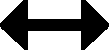
\includegraphics[width=0.5cm]{flechedouble}
}

\newcommand*{\itemperso}{\includegraphics[width=0.8em]{item}}
\newcommand{\xvec}{\mathbf{x}}
\newcommand{\xiivec}{\mathbf{x_i}}
\newcommand{\xjjvec}{\mathbf{x_j}}
\newcommand{\xpvec}{\mathbf{x'}}
\newcommand{\wvec}{\mathbf{w}}
\newcommand{\betavec}{\mathbf{\beta}}
\newcommand{\alphavec}{\mathbf{\alpha}}
\newcommand{\xivec}{\mathbf{\xi}}


\renewcommand{\complex}[1]{\mbox{$\mathcal{O}(#1)$}}
%\DeclareMathOperator{\dist}{d}
\DeclareMathOperator{\sub}{\# sub}
\DeclareMathOperator{\code}{code}
\DeclareMathOperator{\struct}{struct}
\DeclareMathOperator{\myminimize}{minimize}
\DeclareMathOperator{\mymaximize}{maximize}
\newcommand{\minimiser}[1]{\underset{#1}{\myminimize}}
\newcommand{\maximiser}[1]{\underset{#1}{\mymaximize}}
%\DeclareMathOperator{\mymin}{min}
%\DeclareMathOperator{\mymax}{max}
\newcommand{\vecmath}[1]{\mathbf{#1}}

\newcommand*{\itemplus}{
\includegraphics[width=0.8em]{plus}}
\newcommand*{\itemdanger}{\includegraphics[width=1em]{warning}}
\newcommand*{\itemmoins}{
\includegraphics[width=0.8em]{moins}}

\renewcommand{\H}{\ensuremath{\mathcal{H}}}

\newcommand{\myinf}{
  
\includegraphics[width=0.4cm]{inf}
}
\newcommand{\myinfbar}{
  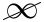
\includegraphics[width=0.4cm]{infbar}
}

\newcommand{\beginbackup}{
   \newcounter{framenumbervorappendix}
   \setcounter{framenumbervorappendix}{\value{framenumber}}
}
\newcommand{\backupend}{
   \addtocounter{framenumbervorappendix}{-\value{framenumber}}
   \addtocounter{framenumber}{\value{framenumbervorappendix}} 
}

\usefonttheme[onlymath]{serif}


\institute{INSA Rouen Normandie - Laboratoire LITIS}

% =================================================================================
\begin{document}
\maketitle

\section{Introduction}
\label{sec:org1f84628}
\begin{frame}[allowframebreaks]{Classification}
  \begin{block}{Principle}
    Identify the category of an object
    \begin{itemize}
    \item Binary classification: Positive or Negative, ${0,1}$ or
      ${-1,1}$ (Breast Cancer,Spam detection, \dots)
    \item Multi classification: More than 2 classes (object
      classification, iris: plant species, \dots) 
    \end{itemize}
  \end{block}

  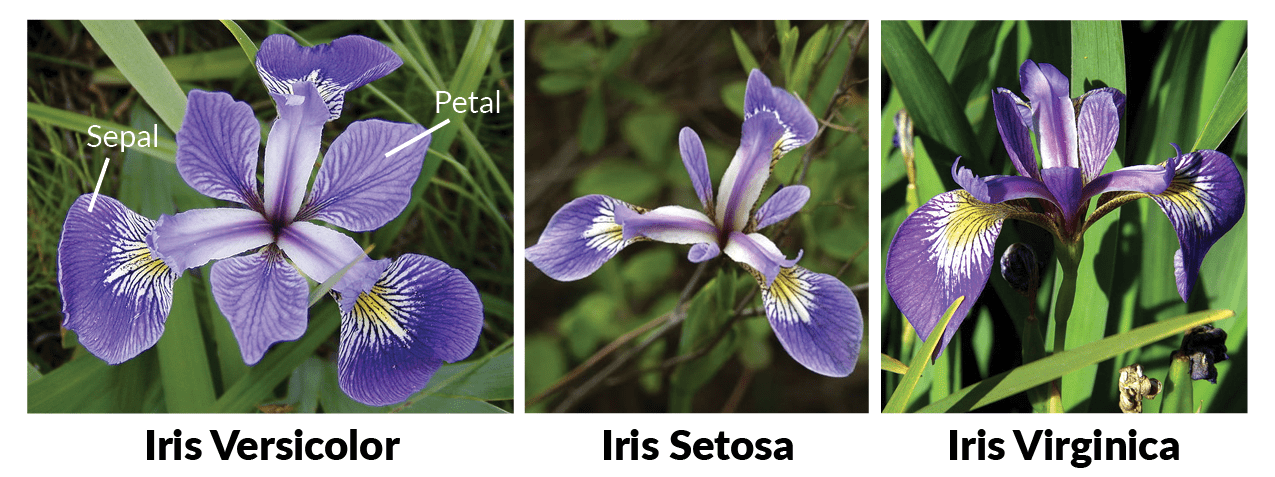
\includegraphics[width=0.45\textwidth]{iris}
  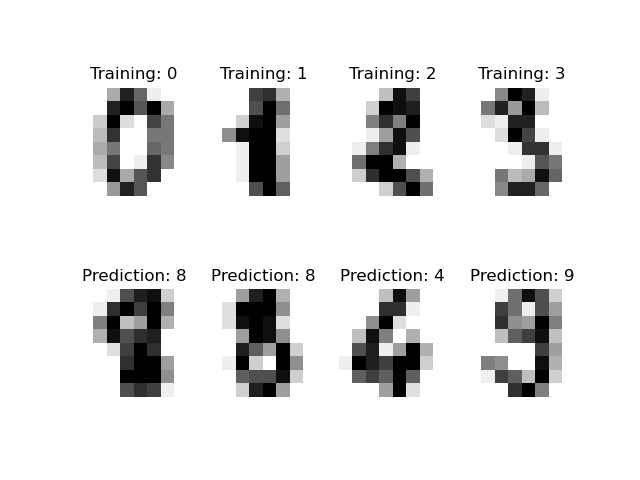
\includegraphics[width=0.45\textwidth]{digits}

  \framebreak 
  \begin{block}{Formally}
    \begin{itemize}
    \item Dataset $\clD = \{(\x_i,y_i) \in \clX \times \clY\}_{i=1 \dots
        N}$ with $\clY \in \{-1,1\}$
    \item Prediction function $f$:
      \begin{itemize}
      \item $f : \clX \to \{-1,1\}$
      \item  $f : \clX \to \R:
        \begin{cases}
          f(\x) > 0 \to 1 \\
          f(\x) < 0 \to -1
        \end{cases}$
      \end{itemize}
    \item Metrics: Accuracy, precision, recall, AUC, \dots 
    \end{itemize}
  \end{block}
\end{frame}
\begin{frame}{Linearly separable problem}
  \begin{block}{}
  It exists  at least one line which separates the data in two classes (in 2D)
  
  \begin{center}
    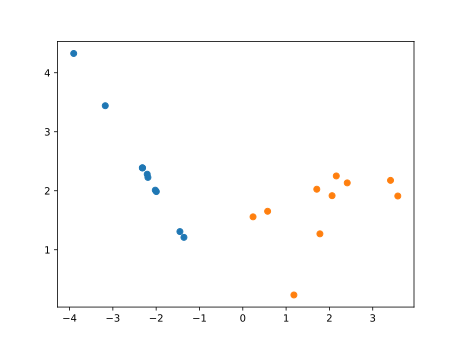
\includegraphics[width=.6\textwidth]{linear_separable}
  \end{center}
  \end{block}
  \end{frame}

 
 \begin{frame}{Linear Classifier}
   \centering{
     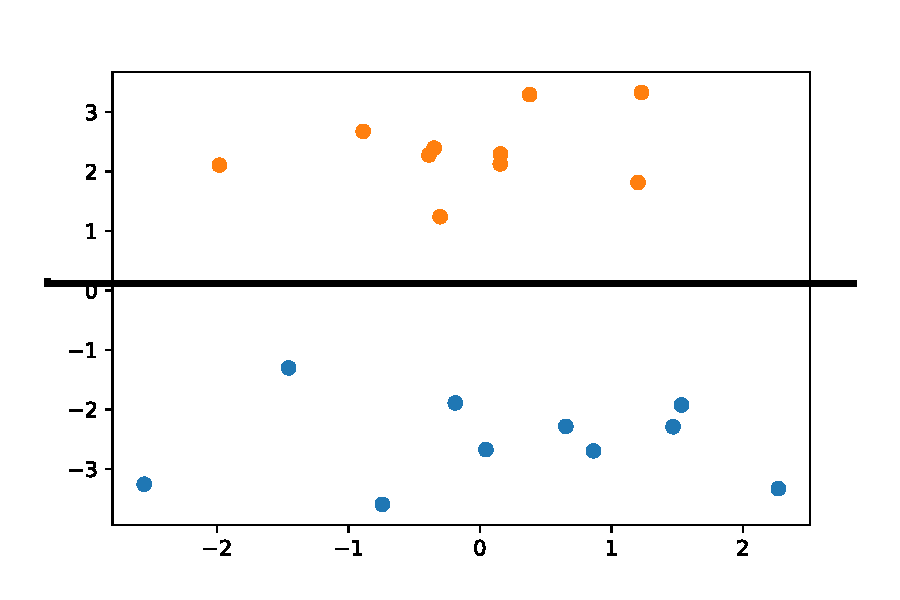
\includegraphics[width=.6\textwidth]{linear_separable_classifier.pdf}
   }
   \begin{itemize}
   \item Find a separator between classes
   \item  Parameters of model  : $\w \in \R^{d}, b \in \R$
   \item Decision function:
     $$f(\x) = \w^\top \x + b
     \begin{cases}
       f(\x) > 0 \to 1 \\
       f(\x) < 0 \to -1 \\
     \end{cases}
$$
   \end{itemize}
\end{frame}
\section{Margin Formulation}
\label{sec:org48fba1b}
\begin{frame}[label={sec:org6952ba1}]{Hyperplane}
  Hyperplane $\clH_{\w,b}$ :
  $$\clH_{\w,b} = \{\z \in R^{d} | 
  f(\z) = \w^\top \z +b = 0 \}
  $$
  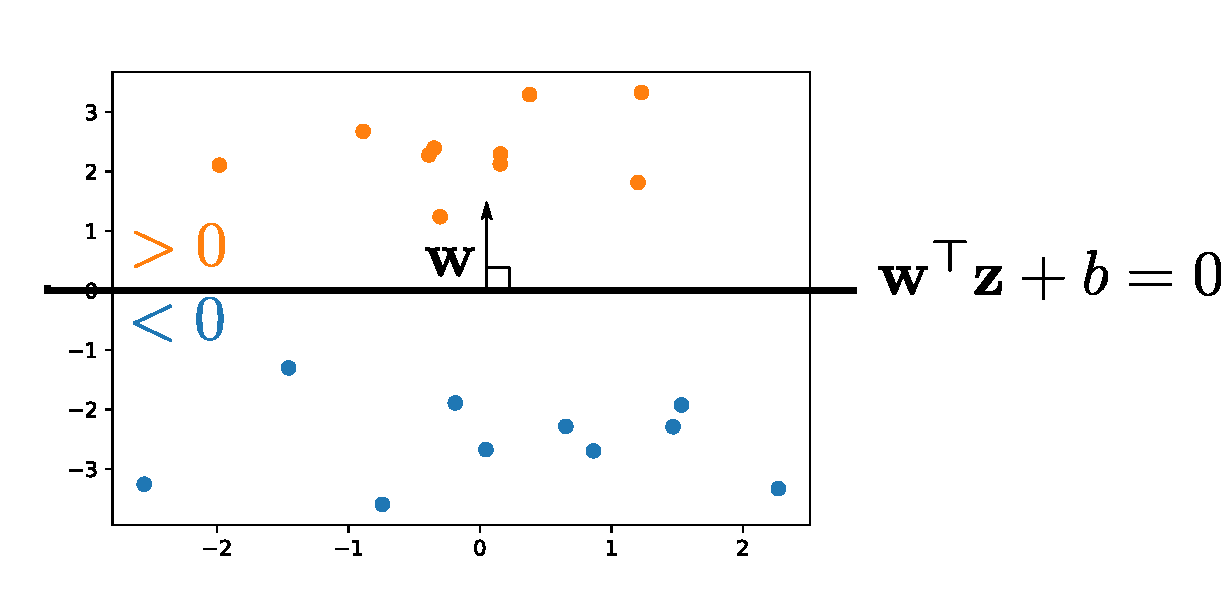
\includegraphics[width=.8\textwidth]{linear_separable_hyperplane}
\end{frame}
\begin{frame}[label={sec:orgd9ceaee}]{Distance to the hyperplane}
  \begin{columns}
    \begin{column}{.6\textwidth}
      \begin{center}
        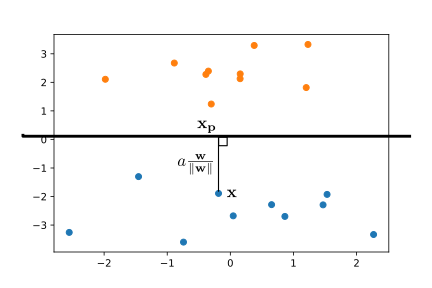
\includegraphics[width=\textwidth]{linear_separable_distance}
      \end{center}
    \end{column}
    \begin{column}{.4\textwidth}
      \begin{eqnarray*}
        &  \x & = \x_p + a \frac{\w}{\|\w\|} \\
        \Rightarrow & a & = \frac{\w^\top \x + b}{\| \w \|}
      \end{eqnarray*}
      \href{https://drive.google.com/file/d/1fGQUw8QEzcfmolNy9gDlvddfdILiAFsO/view?usp=sharing}{Proof}
    \end{column}
  \end{columns}
  \begin{block}{Distance $d(\clH,\x)$}
    \begin{center}
    $$d(\clH,\x) = |a| = \frac{|\w^\top \x + b|}{\| \w \|}$$
  \end{center}

  \end{block}
\end{frame}

\begin{frame}[label={sec:org0f58461}]{Definition of margin}
  \begin{block}{Margin}
    \begin{itemize}
    \item Minimum distance between a point and $\clH$
    \item Canonical hyperplane :
      $$
      \min_{\x_i \forall i \in 1\dots N} \w^\top {\x_i} + b = 1
      $$
    \end{itemize}
    \begin{center}
      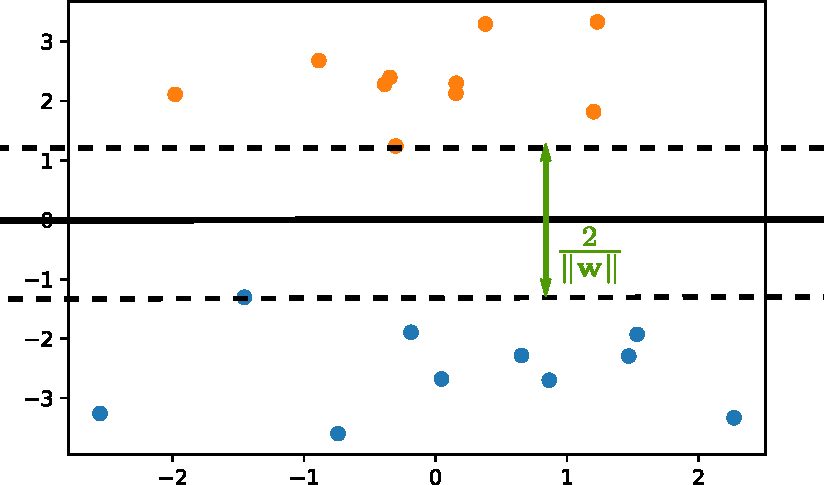
\includegraphics[width=.6\textwidth]{linear_separable_margin}
    \end{center}
  \end{block}
\end{frame}
\begin{frame}{Maximization of margin}
  \begin{block}{Better classifier separates the data}
    \begin{itemize}
    \item Many different hyperplanes separate the data
    \item How to select the best ?
    \item $\Rightarrow$ Maximize the margin
    \end{itemize}
  \end{block}
  \begin{block}{Maximization of the margin}
    \begin{itemize}
    \item Maximize the margin $\Leftrightarrow$ maximize $ \frac{2}{\| \w
        \|}$
    \item $\w^\star = \argmin_\w \| \w \|$ 
    \end{itemize}
  \end{block}
  \framebreak
  \begin{columns}
    \begin{column}{.47\textwidth}
      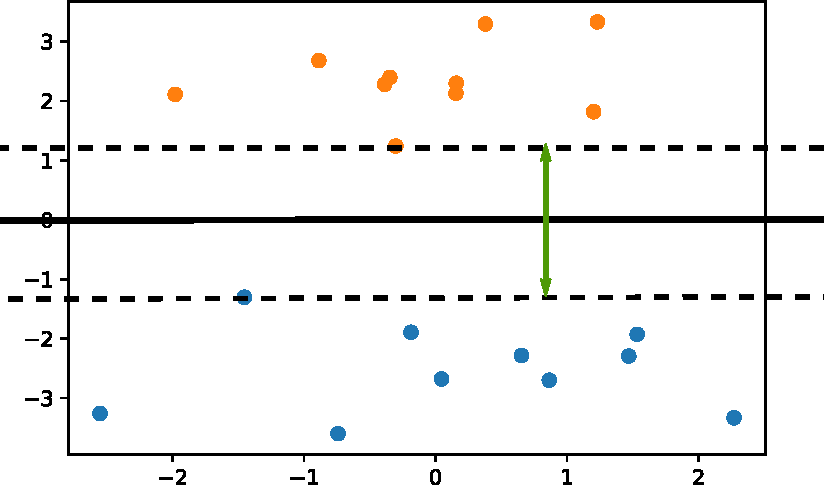
\includegraphics[width=\textwidth]{linear_separable_h1}
    \end{column}
    %\hspace{.5cm}
    \begin{column}{.47\textwidth}
      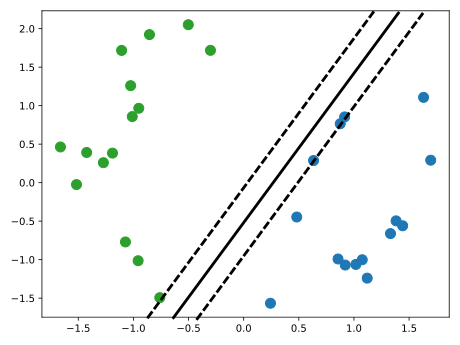
\includegraphics[width=\textwidth]{linear_separable_h2}
    \end{column}
  \end{columns}
  
\end{frame}
\section{Linear Separable SVM}
\begin{frame}[plain]
  \centering{{\huge Linear Separable SVM}}
\end{frame}
\label{sec:orge152145}
\begin{frame}{Principle of SVM}
  Find an hyperplane $\clH$ which :
    \begin{itemize}
    \item separates well the data
      $$
      y_i f(\x_i) > 1, \forall i \in 1 \dots N
      $$
    \item maximizes the margin
      $$
      \argmin_\w \| \w \|^2
      $$
    \end{itemize}
    \centering{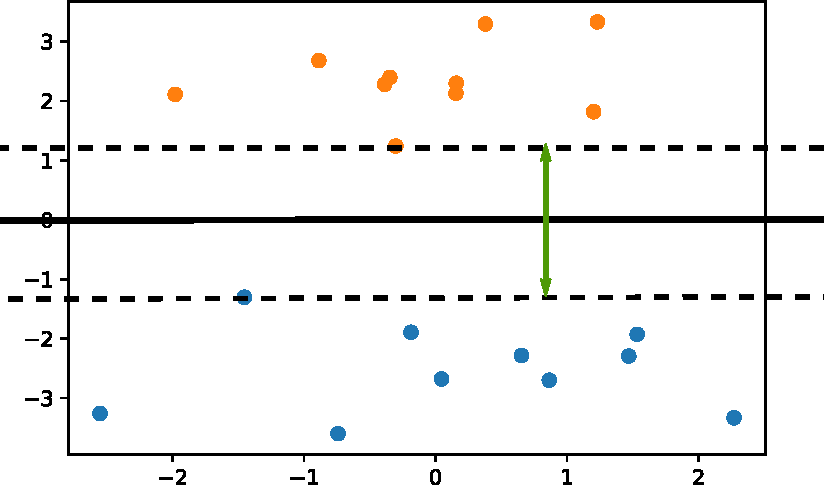
\includegraphics[width=.6\textwidth]{linear_separable_h1}}
\end{frame}
\begin{frame}[label={sec:orgc76d99b}]{Objective function}
  \begin{block}{Hard-margin}
    \large{
      \begin{center}
        \begin{align*}
          \min_{\w,b}& ~~~~  \frac{1}{2} \| \w \|^2  \\
          \text{s.t.} & \\
          &  y_i(\w^\top \x_i + b) \geq 1, \forall i \in 1 \dots N 
        \end{align*}
  
    \end{center}
  }
\end{block}

\end{frame}
\begin{frame}{Control + data term}
  \begin{block}{Data term}
    \centering{
      $y_i(\w^\top \x_i + b) \geq 1$
    }
  \begin{itemize}
  \item N Constraints
  \item Ensures that the train set is separated
    \end{itemize}
  \end{block}
  \hfill
  \begin{block}{Control term}
    \centering{
      $\| \w \|^2$
    }
    \begin{itemize}
    \item Maximize the margin
    \item Selects the ``best'' model
    \end{itemize}
    
  \end{block}
  
\end{frame}
\begin{frame}{How to resolve the SVM problem ?}
  \begin{block}{Constraints}
    \begin{itemize}
    \item We know how to optimize $\| \w \|^2$
    \item But the constraints ? 
    \end{itemize}
  \end{block}
  \begin{block}{Solution }
    \begin{itemize}
    \item Transform the problem
    \item Use Lagrangian dual
    \end{itemize}
  \end{block}
\end{frame}
\begin{frame}[label={sec:org9300cdf}]{Lagrangian equivalence}
  \begin{block}{Lagrangian}
    \begin{itemize}
    \item Dual formulation of a constrained optimization problem
    \item Transform constraints to term
    \item Introduction of Lagrange multipliers for each constraint
    \end{itemize}
  \end{block}
  \begin{block}{Lagrangian of SVM}
    $$
    \clL(\w,b,\alpha) = \frac{1}{2} \| \w \|^2 - \sum_{i = 1}^N
    \alpha_i (y_i(\w^\top \x_i +b) - 1)
    $$
  \end{block}
\end{frame}
\begin{frame}[allowframebreaks]{Dual problem}
  \begin{block}{Dual SVM problem}
    \begin{itemize}
    \item Annilihate the gradient wrt to primal variables
      % \begin{itemize}
      % \item $
      %   \frac{\partial \clL(\w,b,\alpha)}{\partial b}= 0 \Rightarrow
      %   \sum_i^N \alpha_i \y_i = 0
      %   $
      % \item $
      %   \frac{\partial \clL(\w,b,\alpha)}{\partial \w}= 0 \Rightarrow
      %   \w = \sum_i^N \alpha_i \y_i\x_i
      %   $
      % \end{itemize}
    \item Rewrite $\clL(\w,b,\alpha)$ to eliminate primal variables
    \item Minimizing primal $\Leftrightarrow$ maximizing dual
      \begin{align*}
        \max_{\alpha} & \sum_{i=1}^N \alpha_i - \frac{1}{2} \sum_{i=1}^N
                        \sum_{j=1}^N \alpha_i \alpha_j y_i y_j \x_i^\top \x_j \\
        \text{s. t.}  & \\
                      &\alpha_i \geq 0 , \forall i \in 1 \dots N \\
                      & \sum_{i=1}^N \alpha_i y_i = 0\\
      \end{align*}
    \end{itemize}
  \end{block}
  
  \framebreak

  \begin{block}{Resolving dual formulation}
    \begin{itemize}
    \item Quadratic programming (use a solver)
    \item Compute optimal $\alpha^\star$
    \end{itemize}
  \end{block}
  
  \begin{block}{Dual variables $\alpha$}
    \begin{itemize}
    \item $\alpha^\star \in \R^N$ is the solution of dual SVM
    \item $\alpha_i^\star \neq 0$ for $x_i$ in the margin
    \item $\alpha_i^\star = 0$ else.
          \end{itemize}
  \end{block}
\end{frame}

\begin{frame}[label={sec:orgb19430f}]{Support vectors}
\centering{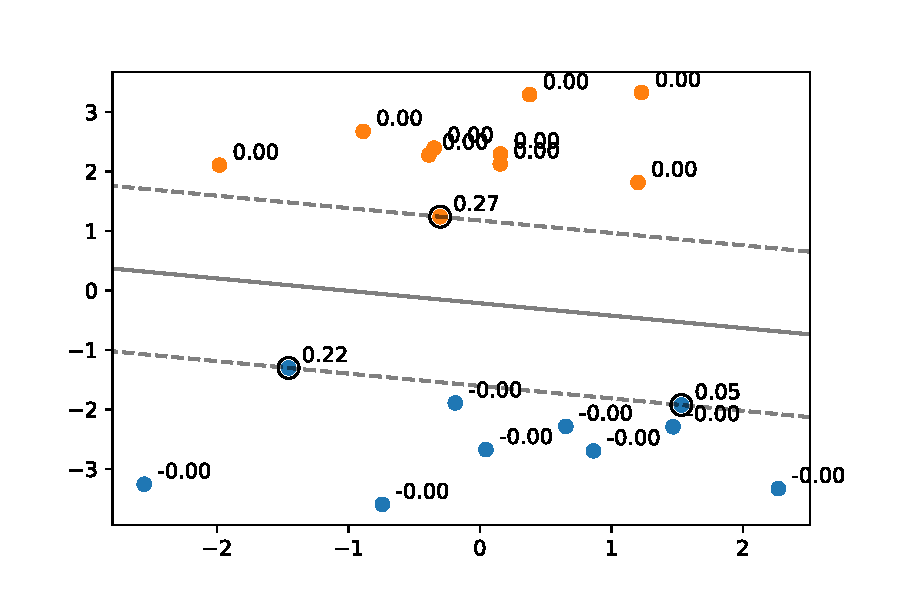
\includegraphics[width=\textwidth]{linear_separable_dual}
}\end{frame}

\begin{frame}[label={sec:org8a8fd9b}]{Classification function}
  \begin{block}{Retrieving $\w$}
    \begin{itemize}
    \item $\w = \sum_{i=1}^N \alpha_i \y_i \x_i$
    \item Decision function $f(\x')$
      $$f(\x') = \w^\top \x' + b = \sum_{i=1}^N
      \alpha_i \y_i \x_i^\top\x' + b$$
    \end{itemize}
  \end{block}
  \begin{block}{Observations}
    \begin{itemize}
    \item No need of $\w$ to predict
    \item Only scalar product between data
    \item Only few support vectors (sparsity)
    \end{itemize}
  \end{block}
\end{frame}
\section{Non separable case}
\begin{frame}[plain]\centering{
  {\Large How to deal with non separable case ?}}
\centering{
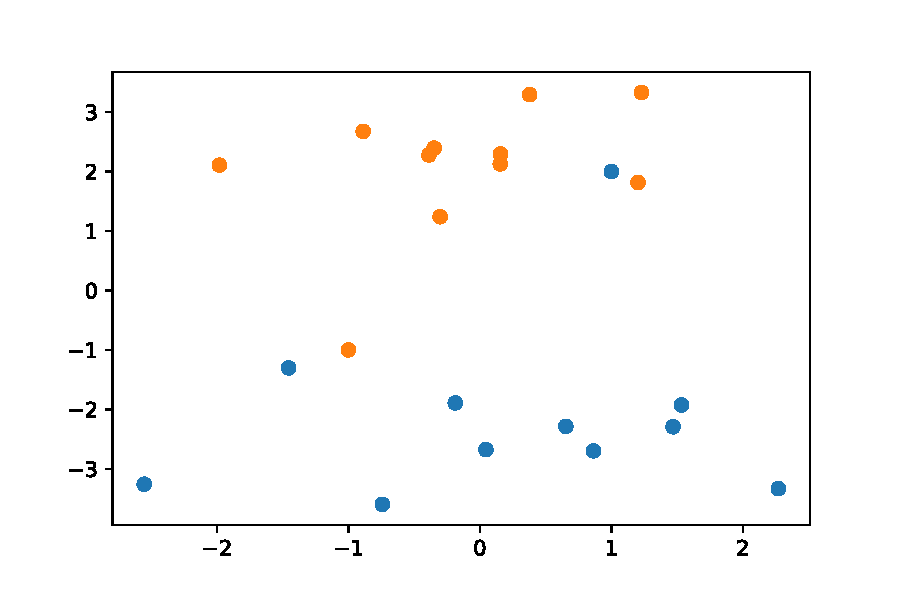
\includegraphics[width=.8\textwidth]{linear_unseparable}}
\end{frame}
\label{sec:orgd1cda88}
\begin{frame}[label={sec:orga7cd2a7}]{The \(\xi\) slack variables}
  \begin{block}{Allow some errors}
    \begin{itemize}
    \item Relax the margin by allowing errors
    \item Constraints:
      $$
      \y_i(\w^\top \x_i +b) \geq 1 - \xi_i
      $$
    \item $\xi_i \geq 0$
    \end{itemize}
  \end{block}
  \begin{block}{Must be minimized}
    \begin{itemize}
    \item Fit to data term
    \item We want to minimize the errors
    \item $\min \sum_i \xi_i$
    \end{itemize}
  \end{block}
\end{frame}
\begin{frame}
  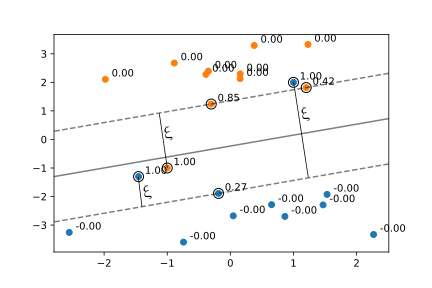
\includegraphics[width=\textwidth]{linear_unseparable_slack}            
\end{frame}

\begin{frame}{SVM-C Objective function}
  \large{
      \begin{center}
        \begin{align*}
          \min_{\w,b}& ~~~~  \frac{1}{2} \| \w \|^2 + C \sum_{i=1}^N \xi_i \\
          \text{s.t.} & \\
          &  y_i(\w^\top \x_i + b) \geq 1 - \xi_i& , \forall i \in 1 
            \dots N \\
          & \xi_i \geq 0 & ,\forall i \in 1 
            \dots N  
        \end{align*}
  
    \end{center}
  }
  \begin{itemize}
  \item $C > 0$
  \item $C$ balances the regularization and fit to data term
  \item Big $C$ : small errors, small margin
  \item Low $C$ : big errors, big margin
  \end{itemize}
\end{frame}
\begin{frame}[plain]
  \begin{centering}
    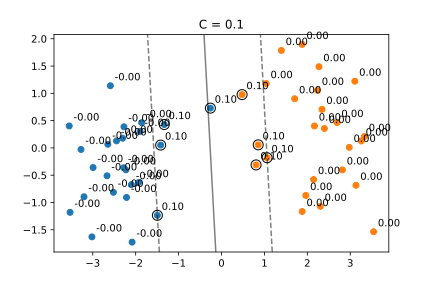
\includegraphics[width=.45\textwidth]{linear_unseparable_C01}
    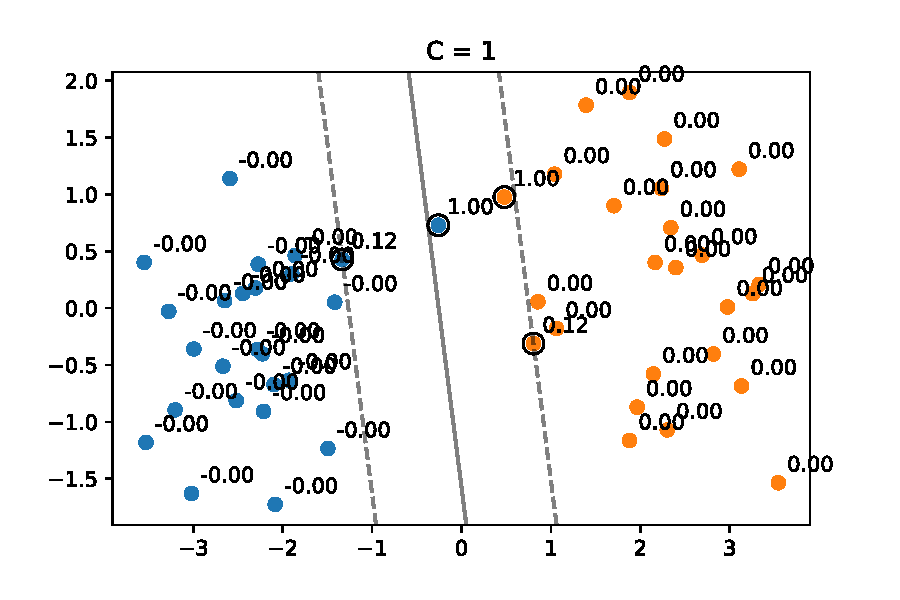
\includegraphics[width=.45\textwidth]{linear_unseparable_C1}
    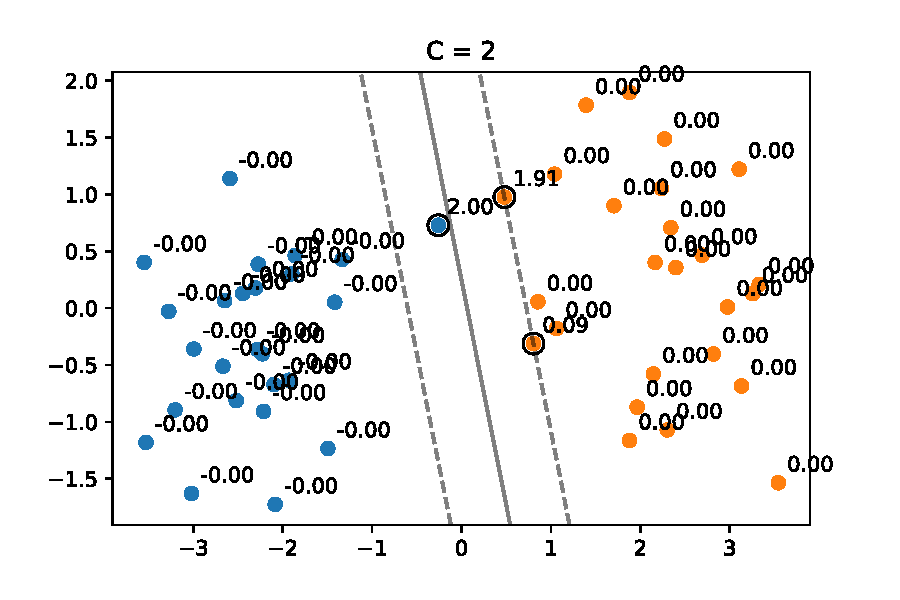
\includegraphics[width=.45\textwidth]{linear_unseparable_C2}
    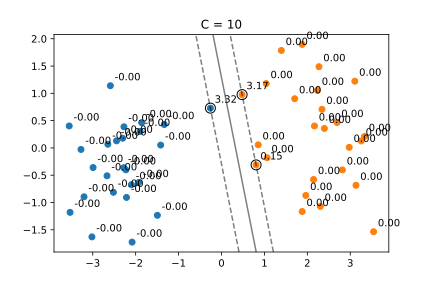
\includegraphics[width=.45\textwidth]{linear_unseparable_C10}
  \end{centering}
\end{frame}
\begin{frame}[label={sec:orga38f76c}]{Dual formulation}
  \begin{block}{Support vector values}
    \begin{itemize}
    \item $0 \leq \alpha_i \leq C$
    \end{itemize}
  \end{block}
  \begin{block}{$C$ parameter}
    \begin{itemize}
    \item Controls the balance regularization/fit to data term
    \item Needs to be tuned
    \end{itemize}
  \end{block}
\end{frame}
\begin{frame}[plain]
  \centering{
  \huge{Let's try it}}
  
\end{frame}

\section{SVM for Regression}
\begin{frame}[plain]
  \centering{\huge{SVM for Regression : SVR}}
  
\end{frame}

\begin{frame}{Regression}
  \begin{block}{Regression problem}
    \begin{itemize}
    \item Dataset $\clD = \{(\x_i,y_i) \in \clX \times \clY\}_{i=1 \dots
        N}$ with $\clY \in \R$
    \item Prediction function $f$:
      $$f(\x_i) = \w^\top \x_i + b \simeq \y_i$$
    \item Metrics: RMSE, MAE, R$^2$, \dots
    \item Methods: Kernel Ridge Regression, \dots
    \end{itemize}
  \end{block}
\end{frame}
\begin{frame}{From classification to regression}
  \begin{block}{How to adapt margin to regression ?}
    \begin{itemize}
    \item We must gather the data 
    \item We don't want to split
    \item How to  ?
    \end{itemize}
  \end{block}
\centering{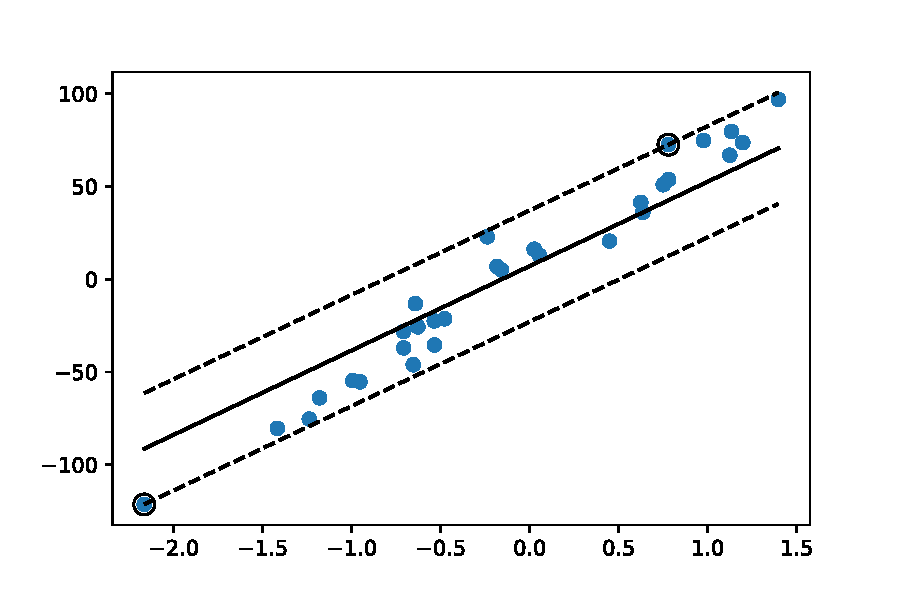
\includegraphics[width=.75\textwidth]{svr_with_epsilon_tube_1}}
\end{frame}
\begin{frame}{Adapting margin to regression}
  \begin{block}{Solution}
    \begin{itemize}
    \item Margin: contains the data
    \item $\w^\top\x_i +b \simeq y_i \Leftrightarrow  \w^\top\x_i +b
      = y_i \pm \varepsilon $
    \item Adapt the size of margin $\varepsilon$ to contain the data
    \end{itemize}
    
  \end{block}
  \begin{center}
    \centering{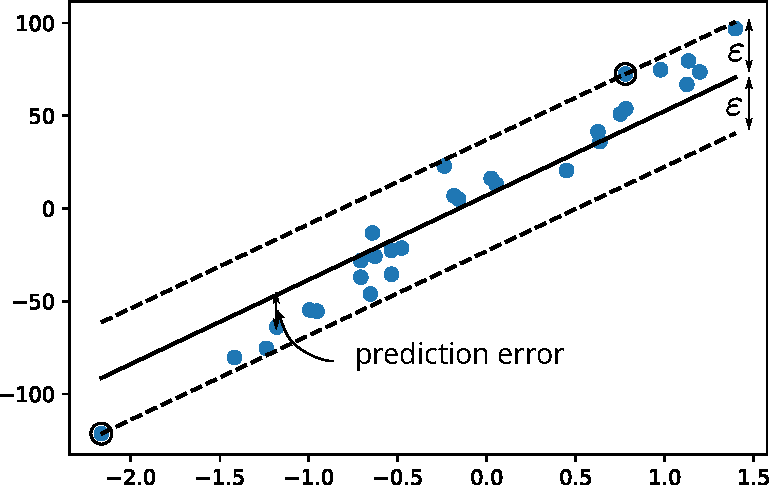
\includegraphics[width=.75\textwidth]{svr_with_epsilon_tube_2}}
  \end{center}

\end{frame}
\begin{frame}{SVR Objective function}
  
  \begin{block}{SVR problem formulation}
    \begin{equation*}
    \begin{aligned}
      \min_{\w,b}\quad  & \frac{1}{2} \| \w \|^2 \\
      \textrm{s t.}\quad & y_i - \w^\top x_i - b \leq \varepsilon,
      \forall i \in 1\dots N \\
      &  \w^\top x_i  + b - y_i \leq \varepsilon,
      \forall i \in 1\dots N                        
    \end{aligned}
  \end{equation*}
  \begin{itemize}
      \item $2 N$ constraints
      \item $\varepsilon$ insensitive cost
    \end{itemize}

  \framebreak
    \begin{block}{Hyperparameters}
      \begin{itemize}
      \item $\varepsilon$ : define the size of the margin
      \item Condition: it exists $\w, b$ which contains the data
        within $\varepsilon$.
      \end{itemize}
    \end{block}
  \end{block}    
\end{frame}
\begin{frame}{Resolution}
  \begin{block}{Dual variables}
    \begin{itemize}
    \item $2N$ dual variables : $\alpha_i, \alpha^\star \geq 0$, 
    \item One vector can be only on one margin 
    \item $\alpha_i \neq 0 \Rightarrow \alpha_i^\star = 0$, and vice
      versa
    \item Constraint satisfied : $\alpha_i^{(\star)} = 0$
    \end{itemize}
  \end{block}
  \begin{center}
    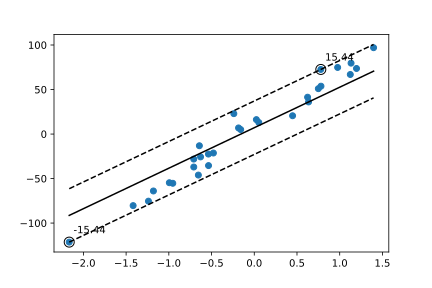
\includegraphics[width=.75\textwidth]{svr_with_epsilon_tube}
  \end{center}

  
\end{frame}

\begin{frame}{SVR with errors}
  \begin{block}{Integrating errors}
    \begin{itemize}
    \item Allowing to be outside the margin
    \item Manage outliers
    \item Relax the constraints with $\xi_i$ values
    \end{itemize}
  \end{block}
  \centering{  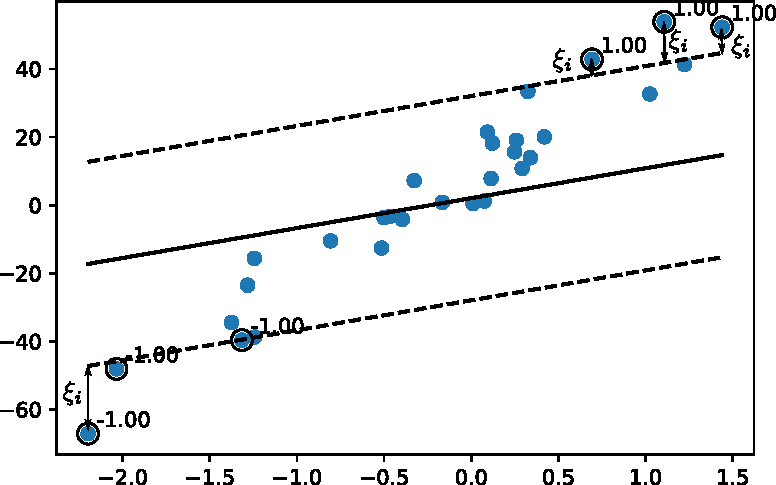
\includegraphics[width=.65\textwidth]{svr_with_epsilon_tube_xi_modif}
  }
\end{frame}

\begin{frame}[allowframebreaks]{SVR objective function}
  \begin{block}{Primal}
     \begin{equation*}
    \begin{aligned}
      \min_{\w,b}\quad  & \frac{1}{2} \| \w \|^2 + C \sum_{i=1}^N
      (\xi_i + \xi_i^\star) \\
      \textrm{s. t.}\quad & y_i - \w^\top x_i - b  \leq \varepsilon + \xi_i&,
      \forall i \in 1\dots N  \\
      &  \w^\top x_i  + b - y_i  \leq \varepsilon + \xi_i^\star& ,
      \forall i \in 1\dots N  \\
      & \xi_i, \xi_i^\star   \geq 0  & ,
      \forall i \in 1\dots N  
    \end{aligned}
  \end{equation*}
\end{block}
\begin{itemize}
\item $4 N$ constraints
\item New hyperparameter: $C \geq 0$
\end{itemize}
\end{frame}
\begin{frame}{Dual Resolution}
  \begin{block}{Dual variables}
    \begin{itemize}
    \item $\alpha_i, \alpha^\star_i$ for errors constraints
    \item $\nu_i, \nu^\star_i$ for positivity on $\xi_i^{(\star)}$
    \end{itemize}
  \end{block}
  \begin{block}{Resolution}
    \begin{itemize}
    \item $\nu_i^{(\star)} = C - \alpha_i^{(\star)}$
    \item $\w = \sum_{i=1}^N (\alpha_i - \alpha_i^\star)\x_i $
    \item $f(\x) = \sum_{i=1}^N (\alpha_i - \alpha_i^\star)\x_i^\top
      \x +b  $
    \end{itemize}
    
  \end{block}
  
\end{frame}

\begin{frame}{$C$ and $\varepsilon$}
  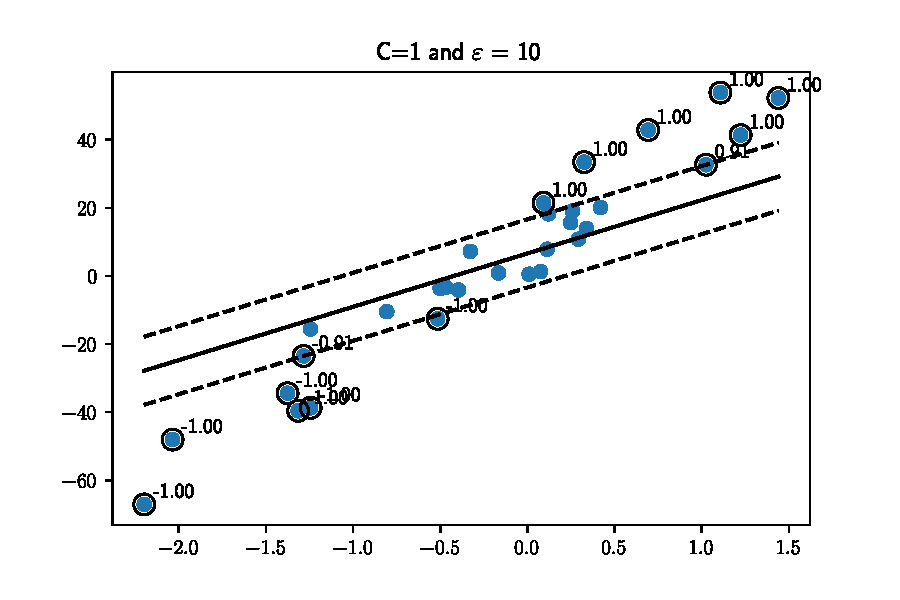
\includegraphics[width=.45\textwidth]{svr_C1_eps10}
  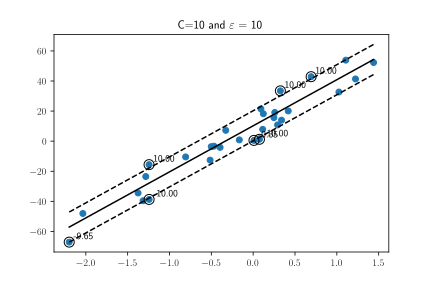
\includegraphics[width=.45\textwidth]{svr_C10_eps10}
  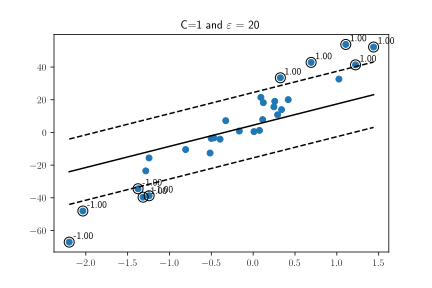
\includegraphics[width=.45\textwidth]{svr_C1_eps20}
  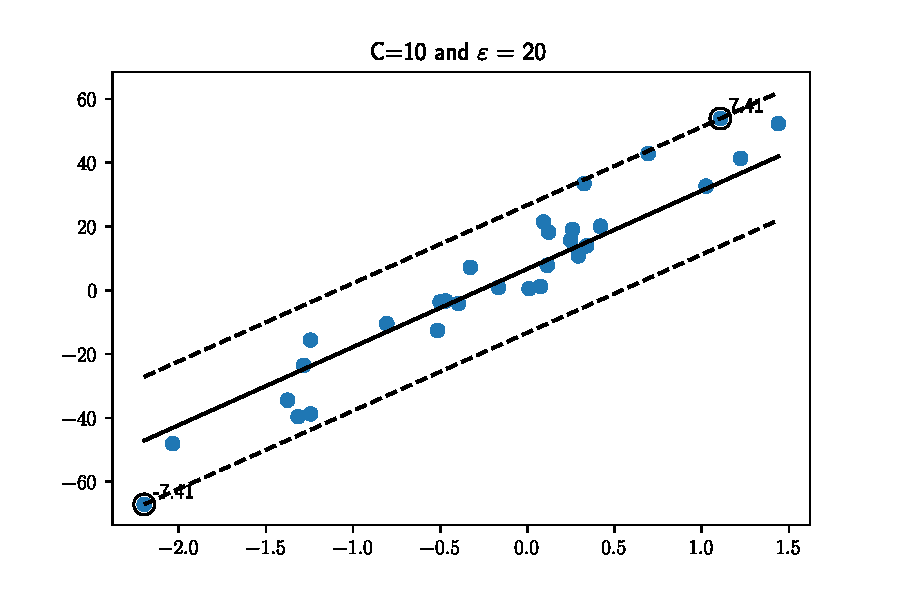
\includegraphics[width=.45\textwidth]{svr_C10_eps20}
  
\end{frame}

%\nocite{*}

\begin{frame}{Others variants of SVM}
  \begin{itemize}
  \item Multiclass formulation: $\clY \in \mathbb{N}$
  \item One class SVM : unsupervised method to detect outliers
  \item $\nu$-SVM : variant of C-SVM
  \end{itemize}

\end{frame}
\begin{frame}[plain]
  \centering{
  \huge{Let's try it}}
  
\end{frame}

\section{Kernel Trick}
%%a faire sauter si pas le temps
\begin{frame}
  \frametitle{Let's revisit SVM}
  
  \begin{block}{Objective function}
    \begin{align*}
      \max_{\alpha} & \sum_{i=1}^N \alpha_i - \frac{1}{2} \sum_{i=1}^N
      \sum_{j=1}^N \alpha_i \alpha_j y_i y_j \x_i^\top \x_j \\
      \text{s. t.}  & \\
      &\alpha_i \geq 0 , \forall i \in 1 \dots N \\
      & \sum_{i=1}^N \alpha_i y_i = 0
    \end{align*}
  \end{block}
  
  \begin{block}{Decision function}
    $$
      f(\x') = \w^\top \x' + b = \sum_{i=1}^N
      \alpha_i \y_i \x_i^\top\x' + b
    $$

  \end{block}
\end{frame}
\begin{frame}
  \frametitle{Observations}
  \begin{block}{What does it mean ?}
    

    \begin{itemize}
    \item Decision function is a linear combination of input data
    \item We don't need explicit data vectors $\x_i$
    \item We only need values of $\langle \x_i, \x_j \rangle, \forall i,j \in
      \{1 .. N\}^2$
    \end{itemize}
  \end{block}

\end{frame}

\begin{frame}
  \frametitle{Observations}
  \begin{block}{Intuition}
    \begin{center}
      By simply modifying the dot product, the algorithm works in another
      space
    \end{center}
  \end{block}

  \begin{block}{This is the \emph{\textbf{Kernel Trick}}}
    \begin{enumerate}
    \item Define your algorithm as it access to data only through scalar
      products
    \item Redefine your scalar product between data by a \emph{kernel}
      $\k(\cdot,\cdot)$
    \item Replace standard scalar product by $\k$
    \item Enjoy
    \end{enumerate}
  \end{block}
\end{frame}

\section{Non linear SVM}
\begin{frame}{Non linear SVM}
  \begin{block}{Linear SVM}
    \begin{center}
          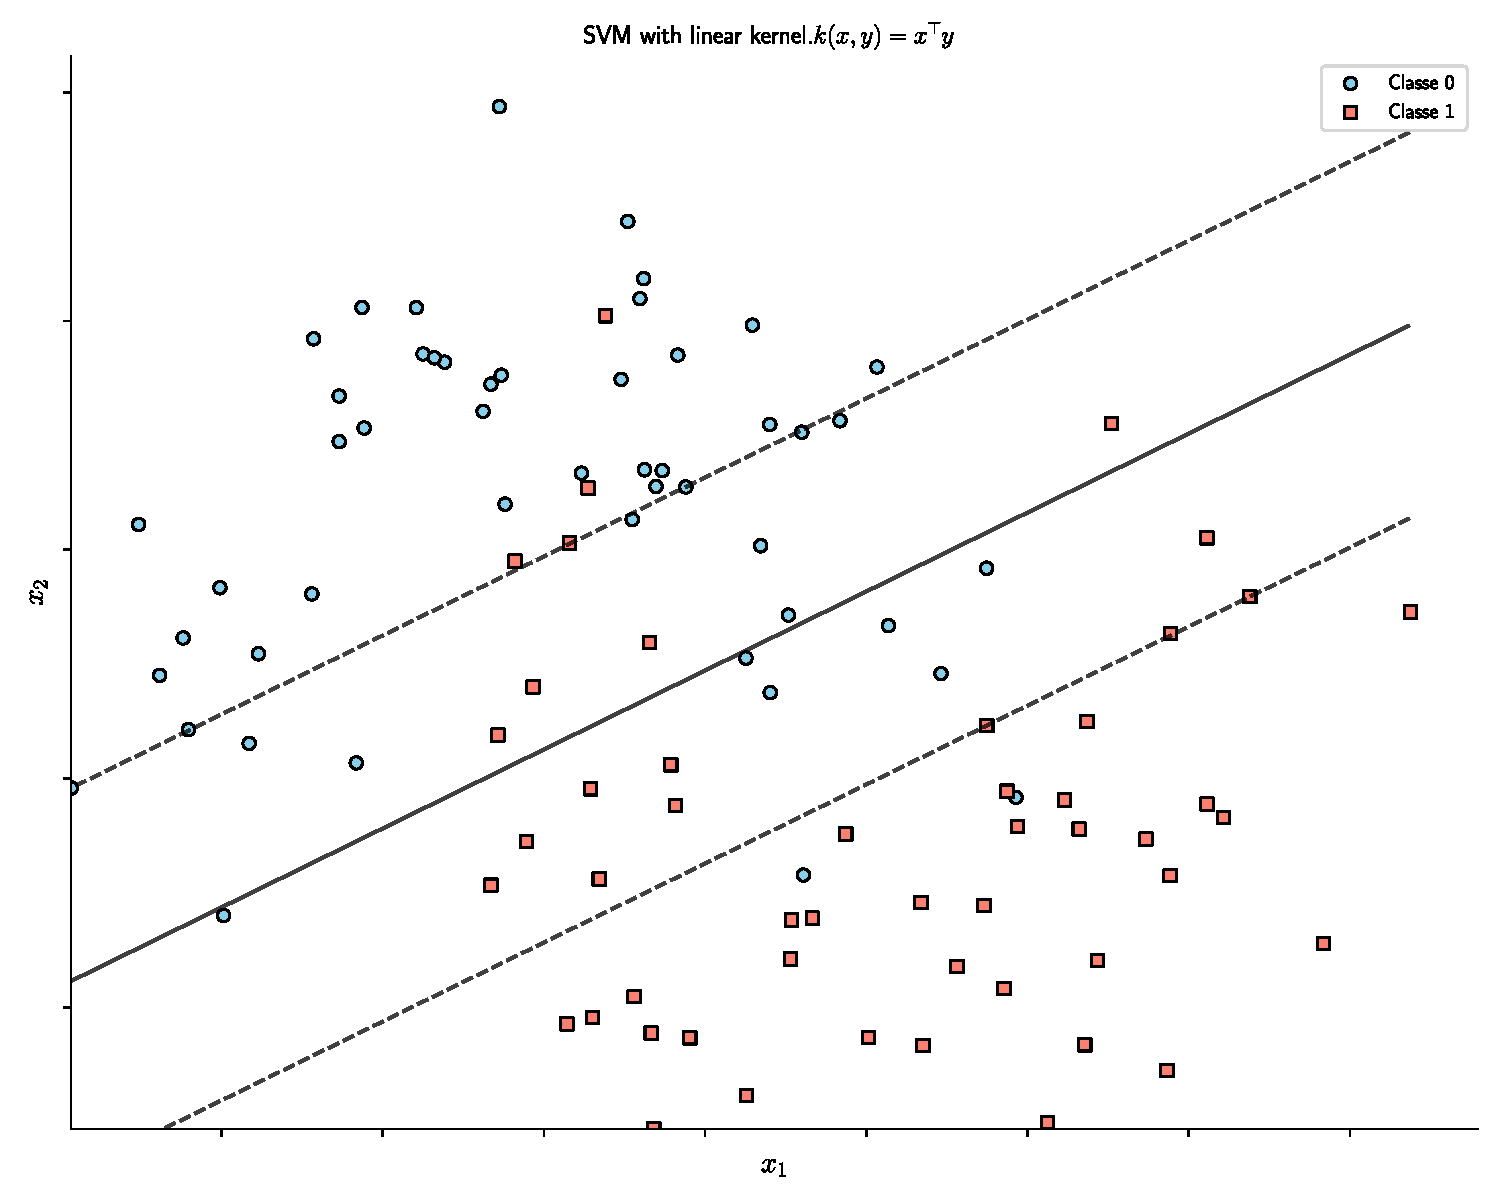
\includegraphics[width=.8\textwidth]{./figures/svm_lineaire.pdf}
    \end{center}
\end{block}

\end{frame}

\begin{frame}{Non linear SVM}
  \begin{block}{Linear SVM}
    \begin{center}
      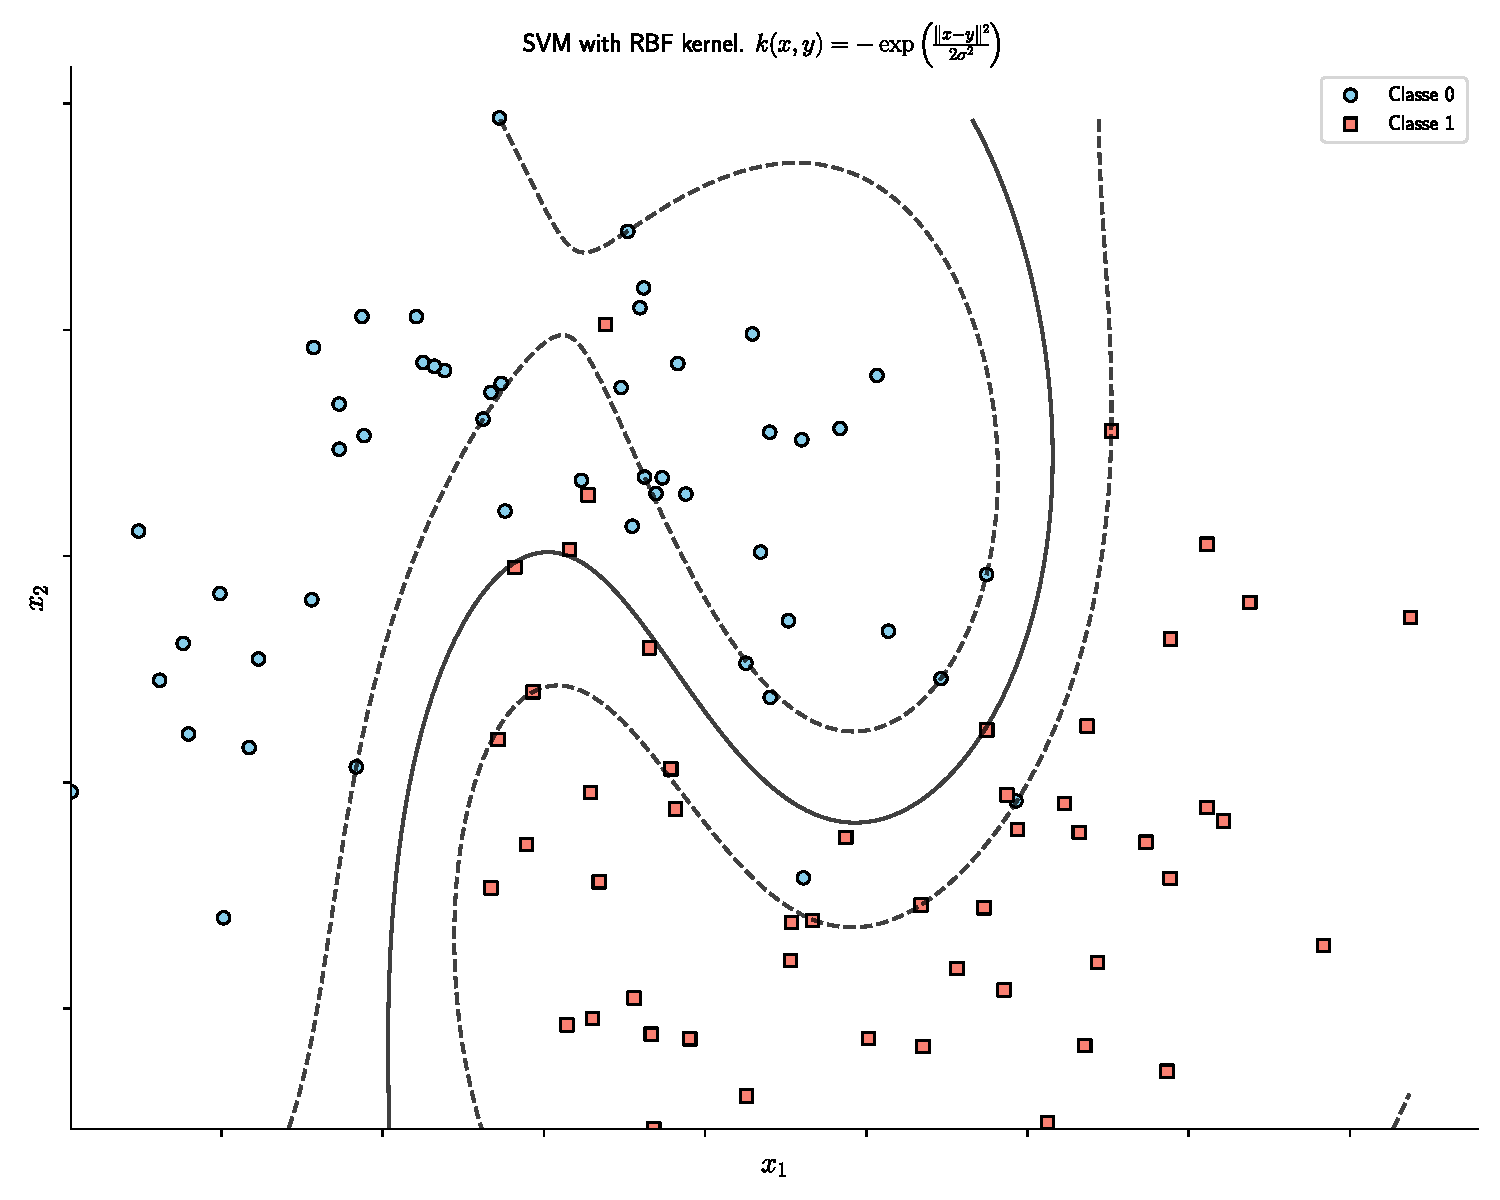
\includegraphics[width=.8\textwidth]{./figures/svm_rbf.pdf}
    \end{center}
\end{block}

\end{frame}
\begin{frame}{Non linear SVM}
  \begin{block}{Linear SVM}
    \begin{center}
          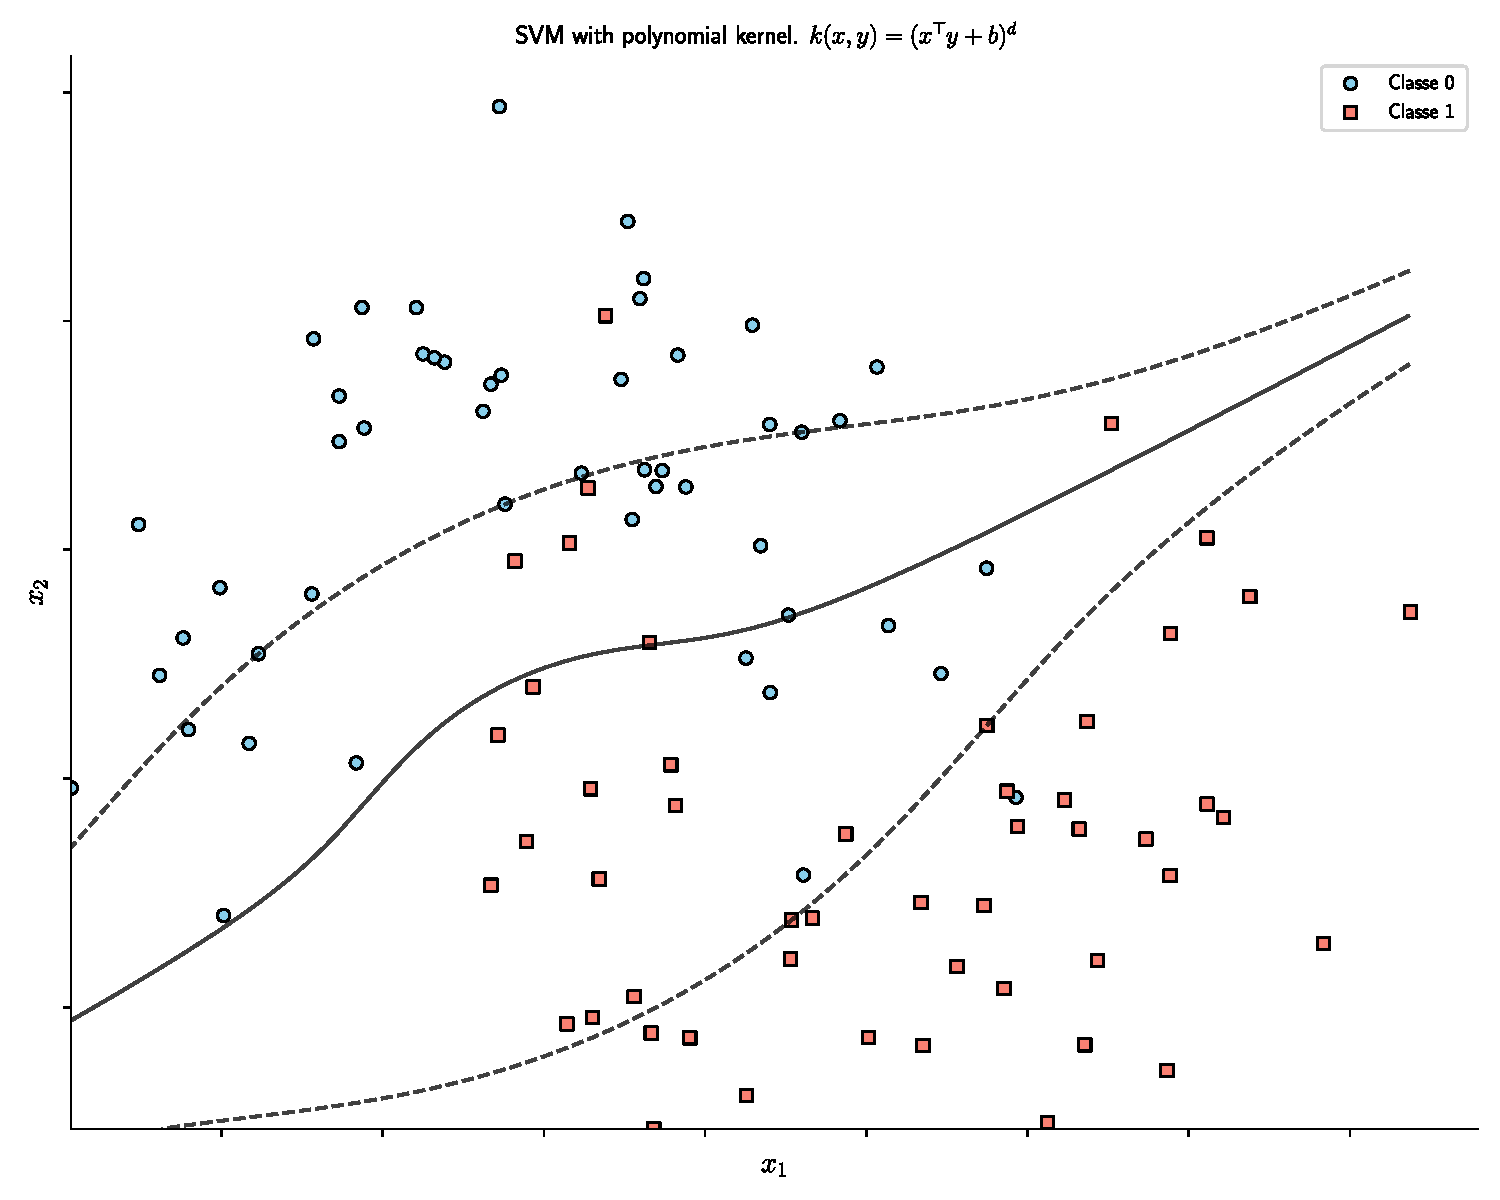
\includegraphics[width=.8\textwidth]{./figures/svm_poly.pdf}
    \end{center}
\end{block}

\end{frame}
\begin{frame}{Non linear SVM}
  \begin{block}{Linear SVM}
    \begin{center}
          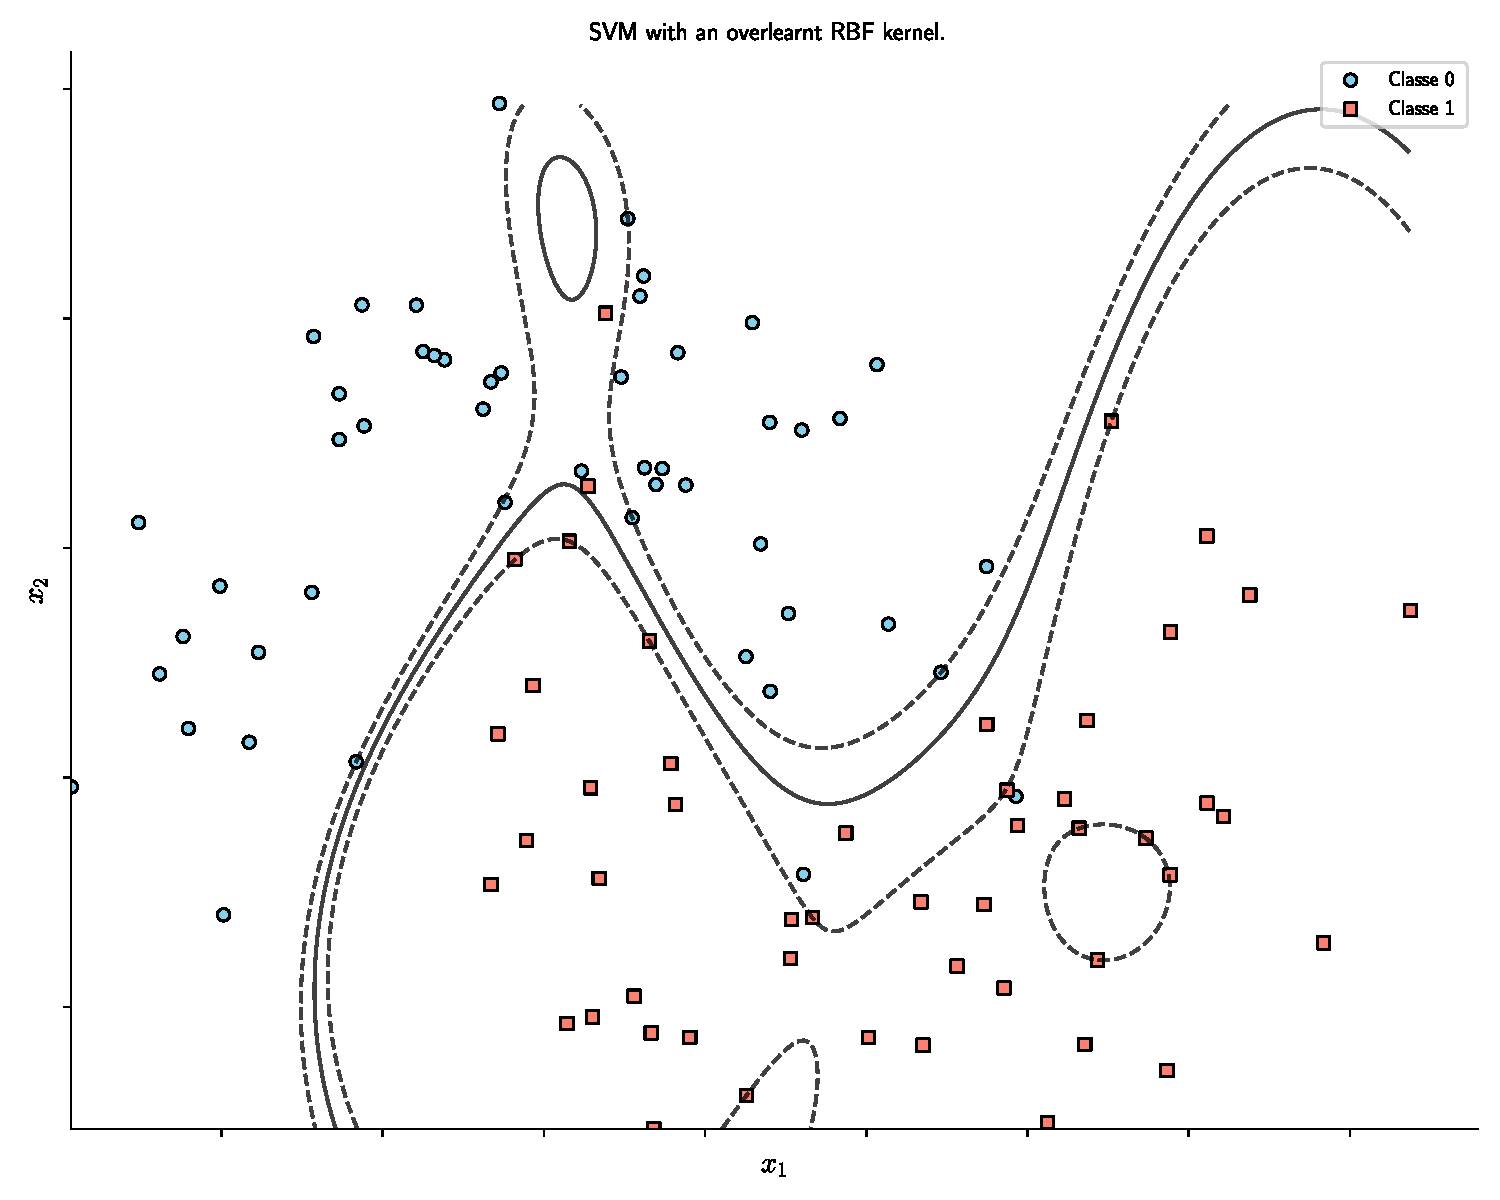
\includegraphics[width=.8\textwidth]{./figures/svm_rbf_overlearning.pdf}
    \end{center}
\end{block}

\end{frame}

\section{Kernels}
\subsection{Theoretical framework}
\begin{frame}[plain]
  \begin{center}
    {\Huge What is a kernel ?}
    
    \vspace{2cm}

    What can be $\k$ ?
  \end{center}
  
\end{frame}

\begin{frame}
  \frametitle{Prerequisites}
  \begin{block}{Some definitions and notations}
    \begin{itemize}
    \item $\clX$: Non empty input space (set of $\dbR^N$, graphs,
      objects, \dots)
    \item $\datax \in \clX$, $\x \in \dbR^d$
    \item $\clH$: feature space with a dot product
      $\langle \cdot, \cdot \rangle_\clH$
    \item $\Phi : \clX \to \clH$: embedding function from $\clX$ to
      $\clH$
    \end{itemize}
  \end{block}
\end{frame}

\begin{frame}
  \frametitle{Kernel}
  {\Large\begin{block}{Definition}
          A kernel $\k$ is a function $\k: \clX \times \clX \to \dbR$:
    {\Huge $$\k(\datax,\datax') = \langle \Phi(\datax), \Phi(\datax') \rangle_\clH$$}
  \end{block}}

%   \footnote{Learning with Kernels, Smola and al.}
\end{frame} 

\begin{frame}
  \frametitle{Positive Definite Kernels}
  \begin{block}{Gram Matrix}
    Given a kernel $k : \clX^2 \to \dbR$, and $\{ \datax_1, \dots,
    \datax_n\} \subseteq \clX$, the corresponding \emph{Gram Matrix} $\K$
    is a $n \times n$ matrix whose elements :
    $$\K_{i,j} \mathrel{\mathop:}=   \k(\datax_i, \datax_j)$$
  \end{block}

  \begin{block}{Positive Semi-Definite Matrix}
    \begin{itemize}
    \item if $\K$ is symmetric and  $\c^T\K\c > 0, \forall \c \neq 0$, K is a positive
      definite matrix
    \item if $\K$ is symmetric and $\c^T\K\c \geq 0, \forall \c \neq 0$, K is a positive
      semi-definite matrix.
    \end{itemize}
    Equivalently:
    $\sum_{i=1}^n \sum_{j=1}^n \c_i \c_j \K_{i,j} \geq 0$
  \end{block}
\end{frame}

\begin{frame}[allowframebreaks]
  \frametitle{Positive Definite Kernels}
  \begin{block}{Definition}
    If for any subset $\clX'\subseteq \clX, |\clX'| = n$, the
    associated Gram Matrix $\K \in \dbR^{n \times n}$ is positive semi-definite, then \emph{$\k$} is a
    \emph{positive definite kernel} on $\clX$.
  \end{block}
  
  \begin{itemize}
  \item Usually, we talk about \emph{kernels}. Positiveness is implicit.
  \item Verifying $\K$ positive semi-definiteness consists in computing
    eigenvalues $ \lambda_1 > \dots > \lambda_n$. if $\lambda_n \geq
    0$, then $\K$ is positive semi-definite.
  \item Keep in mind that $k$ corresponds to a scalar product in $\clH$, so:
    \begin{itemize}
    \item $\k(\datax_i,\datax_j) = \k(\datax_j,\datax_i)$: Then $\K$
      is symmetric.
    \item Consider $\bfX \in \dbR^{n \times d}$, $\K =
      \bfX\bfX^\top$. Eigenvalues $> 0$ follows.
    \end{itemize}
  \end{itemize}
  
\end{frame}
\subsection{Reproducing kernel}

\begin{frame}{Reproducing Kernel Hilbert Space}
  \begin{block}{RKHS}
    \begin{itemize}
    \item $\clH$ is a:
      \begin{itemize}
      \item pre-Hilbert space of functions
      \item endowed with a dot product
      \item and we add a norm
        $\|\f \| := \sqrt{\langle \f, \f\rangle}$
      \end{itemize}

      
    \item  $\clH$ is a Hilbert space.
    
    \item Hilbert space: Generalization of euclidean space to finite or
      infinite dimension
    \end{itemize}
    \begin{center}
      \begin{tcolorbox} {\large $\clH$ is called a \emph{reproducing
            kernel Hilbert space (RKHS)} associated to kernel $\k$ }
      \end{tcolorbox}
    \end{center}\end{block}
\end{frame}

\begin{frame}
  \frametitle{Let's summarize}
  \begin{block}{From kernel to feature space}
    Given a valid kernel $k$, we can associate a RKHS $\clH$ which
    corresponds to the feature space of $\k$.
  \end{block}
  
  \begin{block}{From feature space to kernel}
    Now consider that you have $\Phi : \clX \to \clH$ a mapping function.

    A positive kernel $\k$ is defined by:
    $$ \k(\datax, \datax') = \langle \Phi(\datax), \Phi(\datax') \rangle_\clH$$
  \end{block}

  % a kernel always correspond to a dot product in some space
\end{frame}

\section{Kernel functions}
\subsection{Kernel on vectors}
\begin{frame}[plain]
  \begin{center} {\Huge Kernels in Practice}
  \end{center}

\end{frame}
\begin{frame}
  \frametitle{Linear Kernel}
  \begin{block}{$\k(\s,\t) = \s^\top \t $}
    \begin{itemize}
    \item  $\s,\t\in \dbR^d$
    \item symmetric: $\s^\top \t = \t^\top \s$
      
    \item positive:
      \begin{align*}
        \sum_{i=1}^n \sum_{j=1}^n \alpha_i \alpha_j \k(\x_i,\x_j)
        & = \sum_{i=1}^n \sum_{j=1}^n \alpha_i \alpha_j \x_i^\top \x_j & \\
        & = \left(\sum_{i=1}^n \alpha_i \x_i \right)^\top
          \left(\sum_{j=1}^n \alpha_j \x_j \right) \\
        & = \left\|\sum_{i=1}^n
          \alpha_i x_i \right\|^2
      \end{align*}
    \end{itemize}
  \end{block}
\end{frame}
             
\begin{frame}
  \frametitle{Product kernel}
  \begin{block}{$\k(\datax,\datax') = g(\datax) g(\datax')$}
    \begin{itemize}
    \item $\datax, \datax'\in \clX$
    \item for some $g: \clX \to \dbR$
    \item symmetric: by construction
    \item positive:
      \begin{align*}
        \sum_{i=1}^n \sum_{j=1}^n \alpha_i \alpha_j k(\x_i,\x_j)
        & = \sum_{i=1}^n \sum_{j=1}^n \alpha_i \alpha_j g(\x_i) g(\x_j)  \\
        & = \left(\sum_{i=1}^n \alpha_i g(\x_i)\right)
            \left(\sum_{j=1}^n \alpha_j g(\x_j)\right) \\
        & = \left(\sum_{i=1}^n \alpha_i g(\x_i)\right)^2
      \end{align*}
    \end{itemize}
    \end{block}
\end{frame}


\begin{frame}[allowframebreaks]
  \frametitle{Polynomial kernels}
  \begin{block}{A first approach}
    \begin{itemize}
    \item $\s,\t\in \dbR^N$
    \item All ordered combinations of degree $d$, e.g.:
      \begin{align*}
        \Phi : \dbR^2 \to& \clH = \dbR^4 \\
        (\s_1,\s_2) \mapsto & (\s_1^2,\s_2^2,\s_1\s_2,\s_2\s_1)
      \end{align*}
    \item Dimension of $\clH : \frac{(d+N-1)!}{d! (N-1)!}$
    \item Untractable !
    \end{itemize}
  \end{block}
  \framebreak
  
  \begin{block}{$\k(\s,\t) = \langle \s, \t \rangle^d$, $\s,\t\in \dbR^N$}
    \begin{itemize}
    \item Two valid feature spaces:
    \item All ordered combinations of degree $d$, e.g.:
      \begin{align*}
        \Phi : \dbR^2 \to& \clH = \dbR^4 \\
        (\s_1,\s_2) \mapsto & (\s_1^2,\s_2^2,\s_1\s_2,\s_2\s_1)
      \end{align*}
      \item All unordered combinations of degree $d$, e.g.:
      \begin{align*}
        \Phi : \dbR^2 \to& \clH = \dbR^3 \\
        (\s_1,\s_2) \mapsto & (\s_1^2,\s_2^2,\sqrt{2}\s_1\s_2)
      \end{align*}
    \item Also: $(\s^\T\t + c)^d$, $c \in \dbR^+$.
    \item High dimensional feature space but $\k$ is computed in $\complex{n}$
    \end{itemize}
  \end{block}
  
\end{frame}   


\begin{frame}
\frametitle{Generalisation: finite kernel}
\begin{block}{Embedding}
  \begin{itemize}
  \item Let $\Phi_j$, for $j= {1, \dots, p}$ be a finite dictionary of
    functions $\clX \to \dbR$  (polynomials, wavelets, \dots)
  \item Feature map: 
    \begin{align*}
      \Phi : \clX \to & \dbR^p \\
      \s \mapsto  & \bigl(\Phi_1(\datax),\dots ,\Phi_p(\datax')\bigr)
    \end{align*}
  \item  Linear kernel in the feature space:
    $$
    \k(\datax,\datax') =  \bigl(\Phi_1(\datax),\dots,\Phi_p(\datax)\bigr)^\top
    \bigl(\Phi_1(\datax'),\dots ,\Phi_p(\datax')\bigr)
    $$
  \end{itemize}
  
\end{block}

\end{frame}

\begin{frame}
  \frametitle{Gaussian kernel}
  \begin{block}{$\k(\s,\t) = \exp{\left(-\frac{\|\s - \t\|^2}{2\sigma^2}\right)}$}
    \begin{itemize}
    \item for $\sigma = 1$:
      $$\Phi(\s) =
      \left(
      \frac{
        \exp \frac{\|\s\|^2}{2j}
           }{\sqrt{j!}^{1/j}} \binom{j}{n_1,
        \dots,n_k}^{1/2} \s_1^{n_1} \dots \s_k^{n_k}
    \right)_{j=0,\dots, \infty, \sum_{i=1}^k n_i = j}$$
  \item Feature space has an infinite dimension
  \item Overlearning \smalldanger
  \item $\sigma$ controls the influence area of the kernel
  \item $\sigma$ is another hyperparameter
    
  \end{itemize}
    
  \end{block}
\end{frame}

 \begin{frame}[plain]
 \frametitle{Examples of Gram matrices with different bandwidth}

\vspace{-.3cm}
\begin{center}
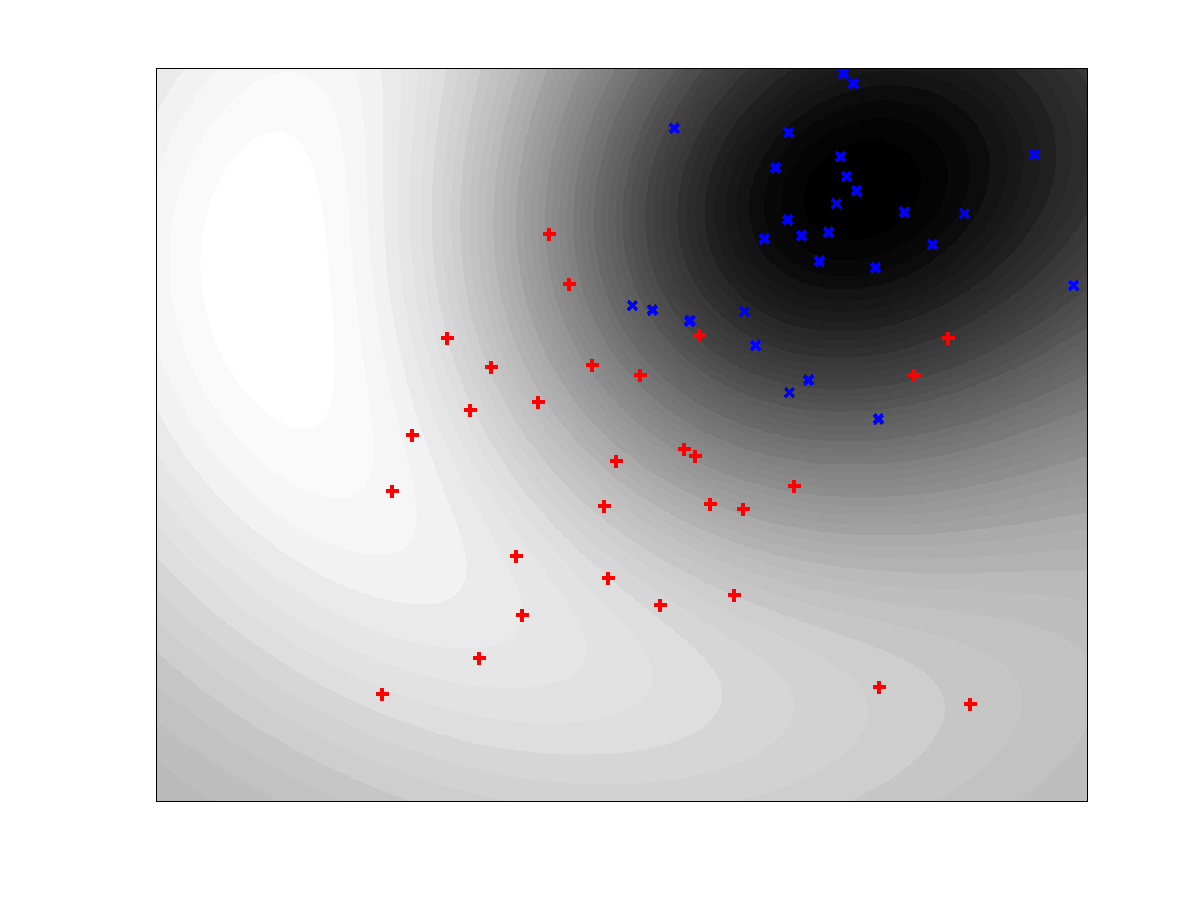
\includegraphics[width=45mm]{Gauss_Gramm_data.png}
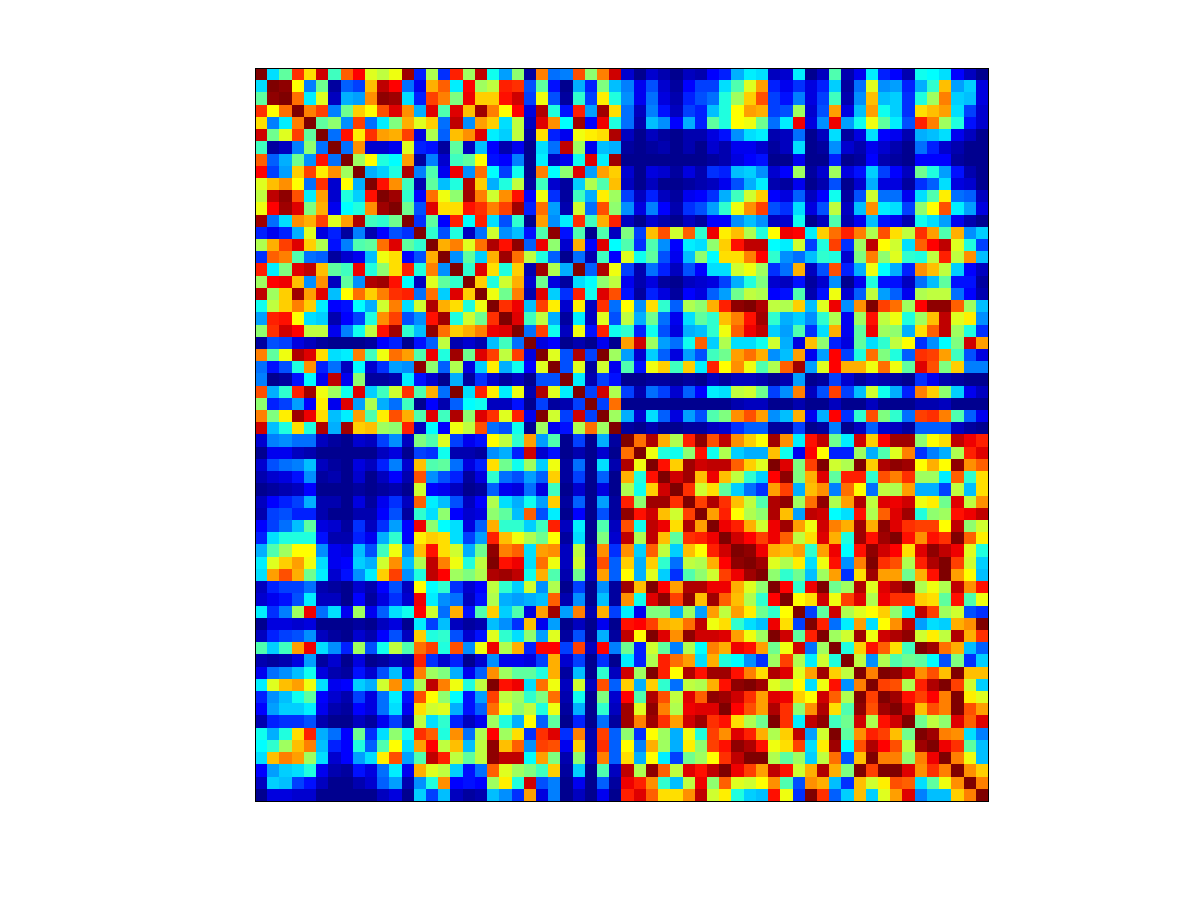
\includegraphics[width=45mm]{Gauss_Gramm_S2.png}

\scriptsize \hfill raw data \hfill Gram matrix for $b = 2 \qquad \qquad \quad $  \hfill 

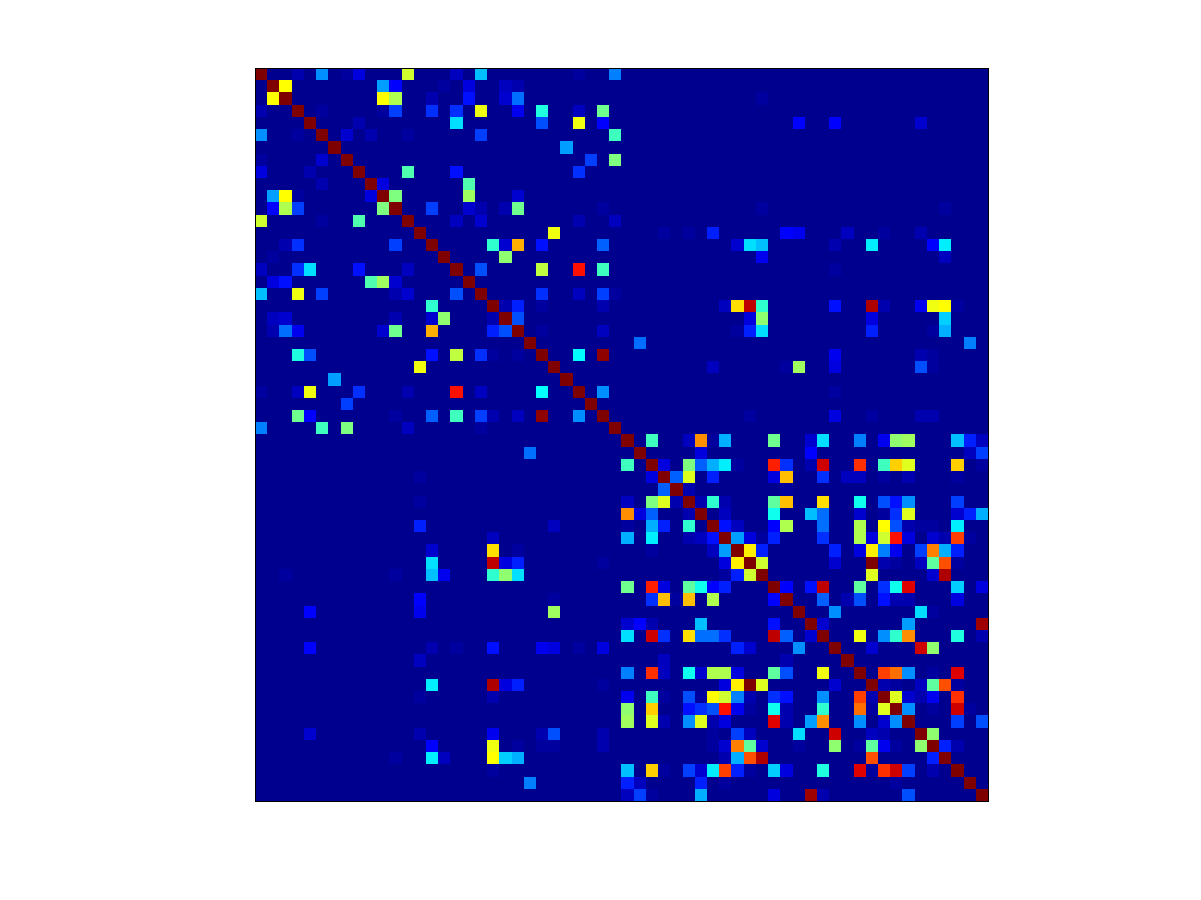
\includegraphics[width=45mm]{Gauss_Gramm_S05.png}
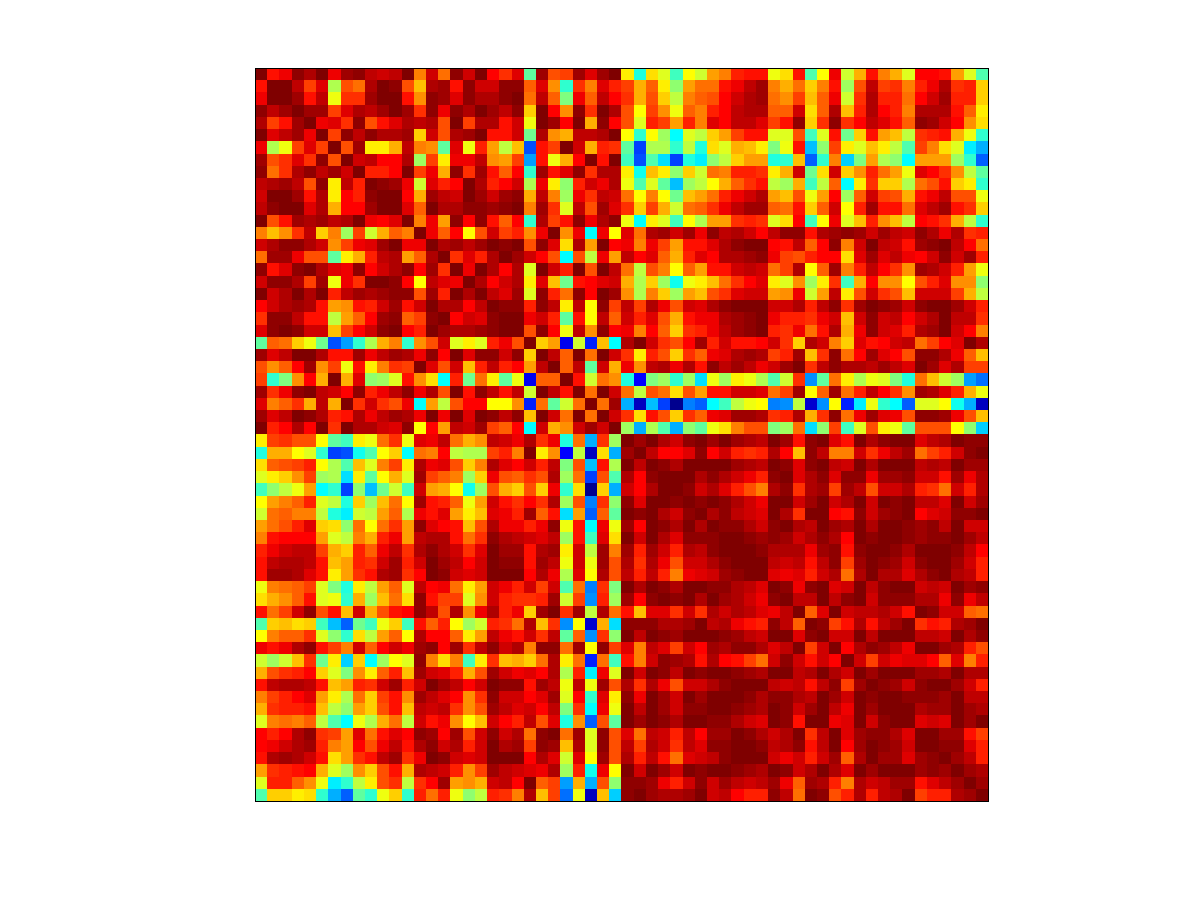
\includegraphics[width=45mm]{Gauss_Gramm_S10.png}

\scriptsize \hfill $b = .5$ \hfill $b = 10\qquad  \qquad  \qquad  \qquad $  \hfill 
\end{center}

 \end{frame} 

% \begin{frame}
%   \frametitle{Histogram kernel}
%   Tanimoto
% \end{frame}

 \subsection{Kernels on generic data}
\begin{frame}
  \frametitle{Kernels on structures}
  % \begin{columns}
  %   \begin{column}{0.3\textwidth}
      \begin{itemize}
      \item $\clX$ may not be a vector space.
      \item we can define kernels on any kind of data :
        
        \begin{itemize}
        \item Strings
        \item Time series
        \item Graphs
        \item Images
        \item \dots
        \end{itemize}
        \end{itemize}

      % \end{column}
      % \begin{column}{0.7\textwidth}
        \begin{center}
          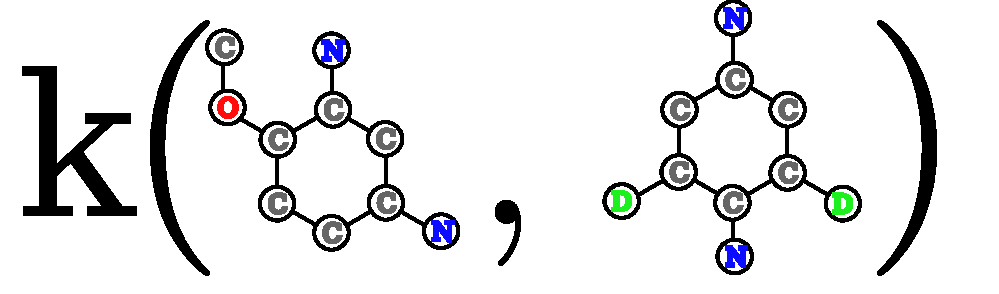
\includegraphics[width=0.8\textwidth]{graph_kernel}
        \end{center}
    %   \end{column}

    % \end{columns}
  \end{frame}

  \subsection{Kernels and distances}
\begin{frame}[allowframebreaks]
  \frametitle{Kernel from distances}
    \begin{block}{Kernel and distance}
  \begin{itemize}
  \item Distance is a dissimilarity measure between vectors or objects
    \begin{align*}
      \dist^2(\s,\t) = &\| \s - \t \|_2^2 \\
      = & (\s - \t)^\top (\s - \t) \\
      = & \s^\top\s + \t^\top\t -2 \s^\top \t \\
      = & \langle \s, \s \rangle + \langle \t, \t \rangle - 2  \langle
          \s, \t \rangle \\   
      = & \k(\s, \s) + \k( \t, \t) - 2 \, \k(\s, \t) \\                    
    \end{align*}
  \item For normalized kernels ($\k(\datax,\datax') = 1$) kernel is
    proportional to the opposite of squared distance
  \item Kernels correspond to similarity measures
  \end{itemize}
\end{block}
\framebreak
\begin{block}{From distance to kernels}
  \begin{itemize}
  \item We can define a kernel from an euclidean distance
  \item Usually we plug a distance in Gaussian Kernel
  \item Use of distance map
    \begin{align*}
      \clX &\to  \dbR^n \\
    \Phi(\datax) &=  ( \dist(\datax,\datax_1), \dots, \dist(\datax,\datax_n))  
    \end{align*}
    
  \item Related to kernel feature map 
  \end{itemize}
\end{block}
\end{frame} 

\begin{frame}
  \frametitle{Kernel jungle}
  \begin{columns}
    \begin{column}{0.5\textwidth}
  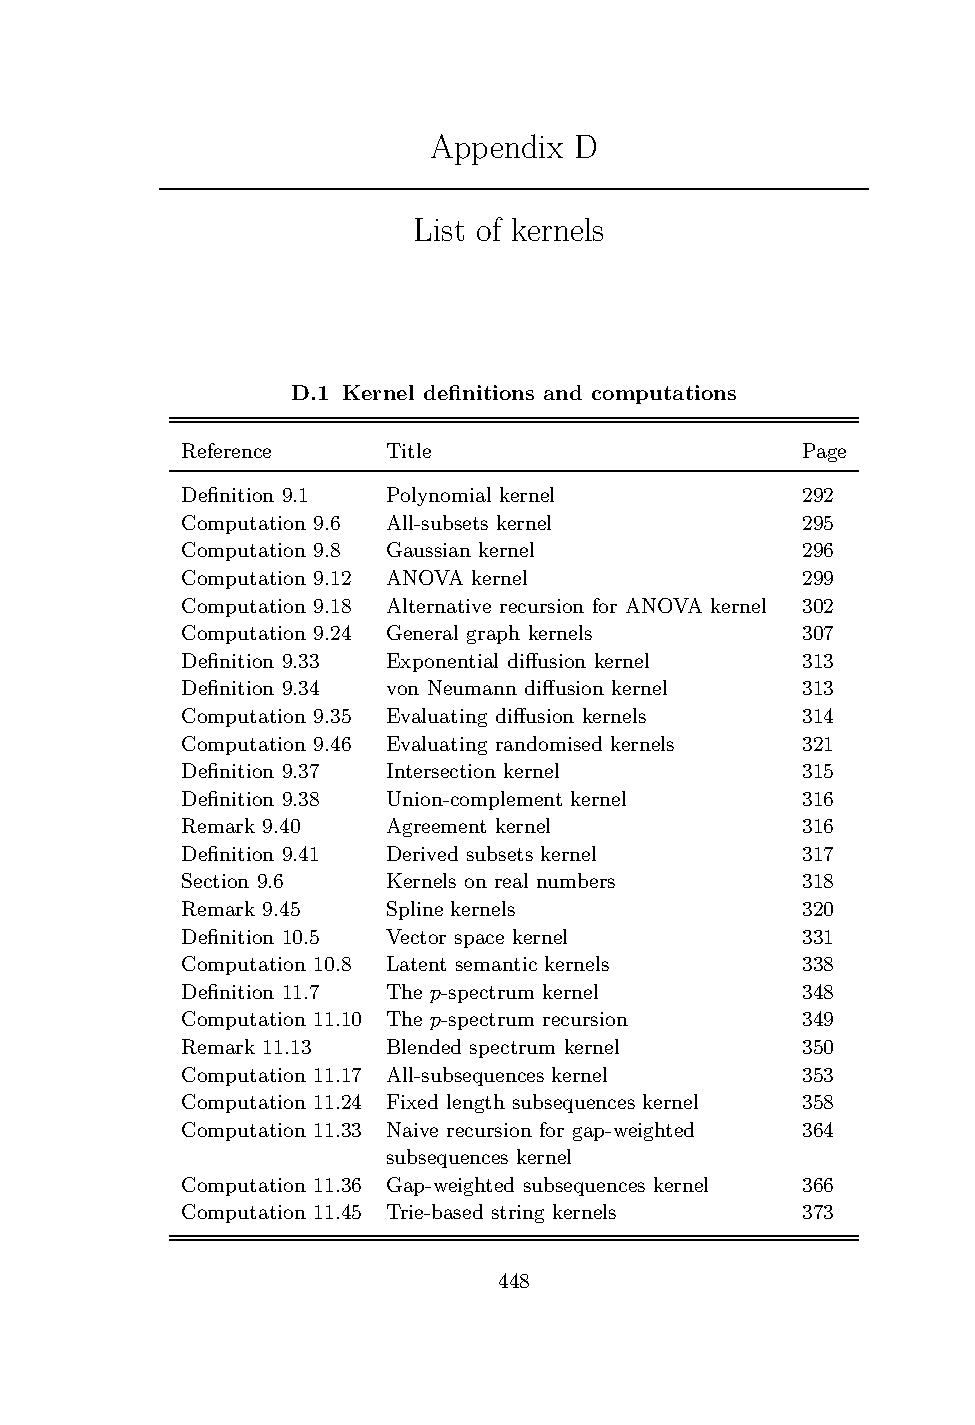
\includegraphics[height=0.8\textheight]{list_kernels_1}
      
    \end{column}
    \begin{column}{0.5\textwidth}
  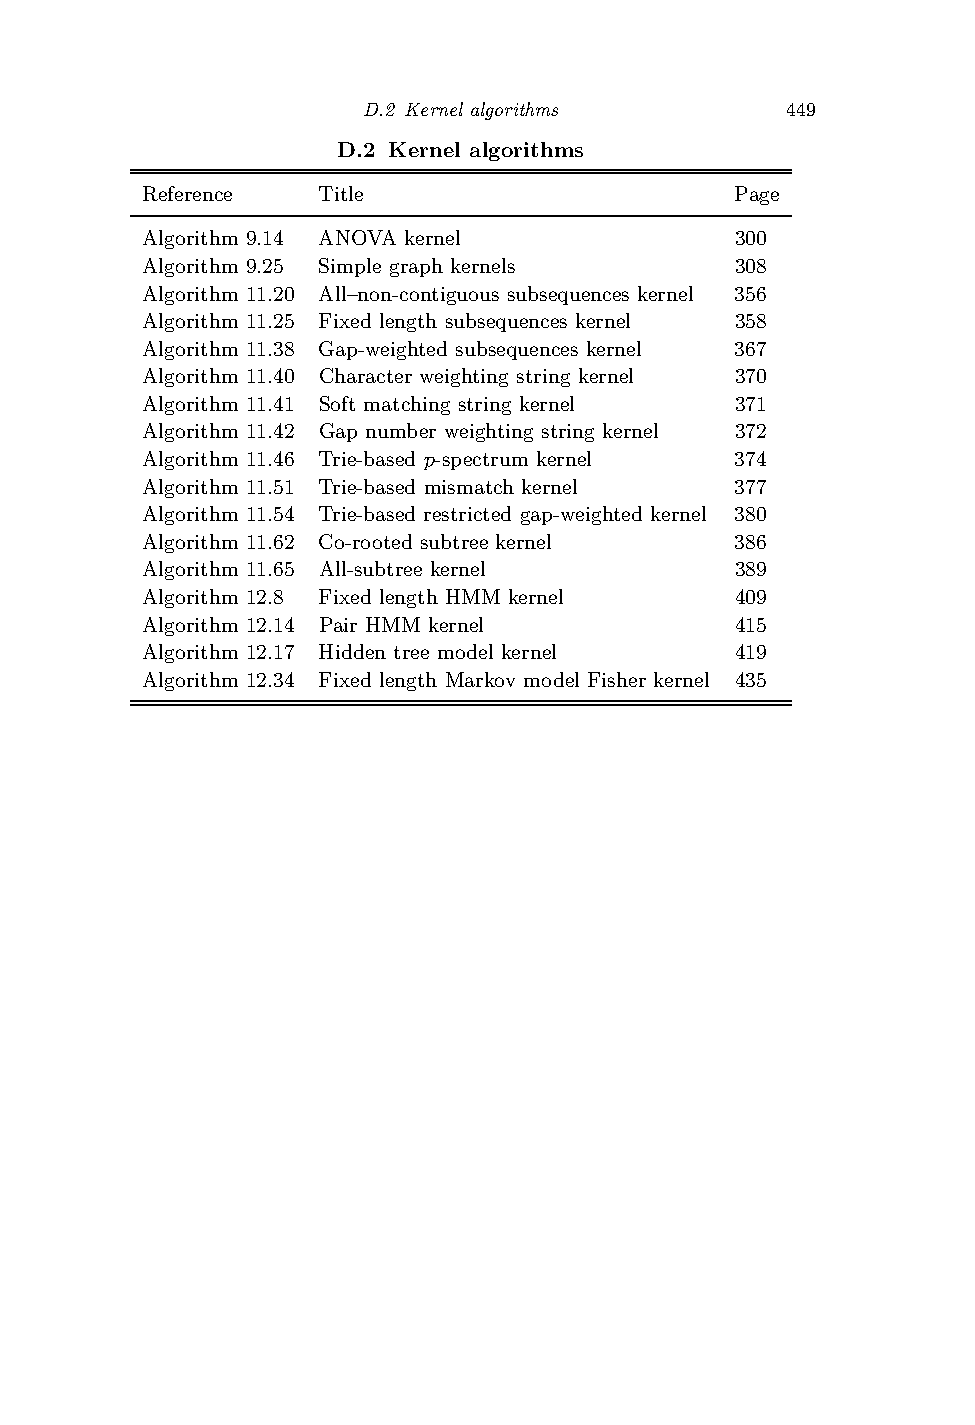
\includegraphics[height=0.8\textheight]{list_kernels_2}
  
    \end{column}
  \end{columns}

 \citep{Shawe-kernel-2004}
\end{frame}  

\begin{frame}
  \frametitle{Invalid kernels}
  \begin{block}{Danger}
    Some similarity measures may be invalid kernels
    \begin{itemize}
    \item $\k(x,y) = \max(x,y)$. 
    \item Optimal assignment kernel:
      \citep{Frohlich05optimalassignment}
    \item and many more \dots
    \item The use is not forbidden, but handle with care
    \item $\to$ operating in Krein spaces: \citep{Loosli13svmin}
    \end{itemize}
  \end{block}
    \begin{center}
    
\includegraphics[width=0.2\textwidth]{danger}
  \end{center}

\end{frame}
\section{Building kernels}
\begin{frame}
\frametitle{Kernel algebra}

%\vspace*{-.15cm}
%think about positive matrices

\begin{block}{Convex cone:}
  The set of kernels forms a convex cone, closed under pointwise
  convergence.


  \vspace{.5cm}
  \begin{itemize}
  \item \textbf{Linear combination}:
    \begin{itemize}
    \item if $\k_1$ an $\k_2$ are kernels, $a_1$,$a_2 \geq 0$, then
      $a_1\k_1 + a_2 \k_2$ is a kernel
    \item if $\k_1$, $k_2$, \dots are kernels, and
      $\k(\datax,\datax') := \lim_{n\to\infty} \k_n(\datax,\datax')$
      exists for all $\datax$, $\datax'$, then $\k$ is a kernel
    \end{itemize}
      \vspace{.5cm}
  \item \textbf{Product kernel}: \\
    if  $\k_1$ an $\k_2$ are kernels, then $\k_1\k_2(\datax,\datax')
    := \k_1(\datax,\datax')\k_2(\datax,\datax')$ is a kernel.  

  \end{itemize}
\end{block}
\end{frame} 

\begin{frame}
  \frametitle{And some molecular graphs kernels}
  \framesubtitle{How to define the similarity between molecules ? }
 \textbf{Graph kernel based on bags of patterns}
  \begin{itemize}
  \item[(1)] \blue{Extraction} of a set of patterns,
  \item[(2)] \blue{Comparison} between \blue{patterns},
  \item[(3)] \blue{Comparison} between \blue{bags} of patterns.
  \end{itemize}

  \begin{center}
    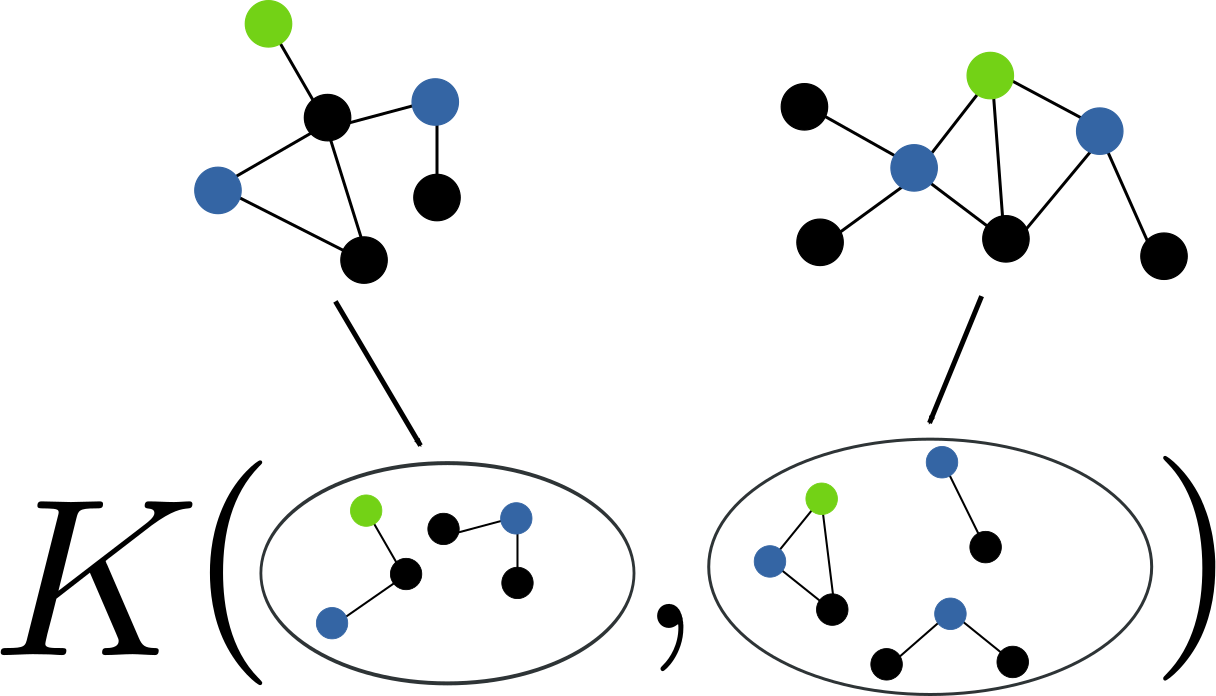
\includegraphics[width=0.5\textwidth]{bags_patterns}
  \end{center}
\end{frame}

\begin{frame}
  \frametitle{Patterns}
  \framesubtitle{Linear Patterns}
  \begin{columns}
    \begin{column}{0.67\textwidth}
      \begin{itemize}
      \item \textbf{Random Walks \hspace{-0.3cm} \myinf \cite{RI-KASHIMA-2003}}
        \begin{itemize}
        \item[\itemmoins] Tottering
        \item[\itemplus]  ~\cite{RI-MAHE-2004}.
        \end{itemize}
        \vspace{.8cm}
      \item \textbf{Paths \hspace{-0.3cm} \myinfbar \cite{RI-RALAIVOLA-2005}}
        \begin{itemize}
        \item[\itemmoins] Low branching description
        \end{itemize}
        \vspace{.8cm}
      \item \textbf{Cyclic patterns \hspace{-0.3cm} \myinfbar \cite{CI-HORVATH-2004}}
        \begin{itemize}
        \item[\itemplus] Cyclic information
        \item[\itemplus] Relevant in chemoinformatics
        \item[\itemmoins] Only a partial cyclic information
        \end{itemize}
        
      \end{itemize}
      
    \end{column}
    \begin{column}{0.32\textwidth}
      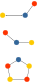
\includegraphics[height=0.6\textheight]{patterns-linear}
    \end{column}
  \end{columns}
  
\end{frame}

\begin{frame}
  \frametitle{Patterns}
  
  \begin{columns}
    \begin{column}{0.67\textwidth}

      \begin{itemize}
      \item \textbf{Graphlets \hspace{-0.3cm} \myinfbar \cite{CI-SHERVASHIDZE-2009}}
        \begin{itemize}
        \item[\itemplus] \blue{Non linear} structures.
        \item[\itemmoins] \blue{Non labeled} patterns.
        \item[\itemplus] Linear complexity.
        \end{itemize}
        \vspace{.8cm}
      \item \textbf{Tree-patterns \hspace{-0.3cm} \myinf
          \cite{RI-MAHE-2009, RI-SHERVASHIDZE-2011}}
        \begin{itemize}
        \item[\itemplus] \blue{Non linear} and \blue{labeled} patterns.
          % \item[\itemplus] Pondération des motifs.
        \end{itemize}
        \vspace{.8cm}
      \item \textbf{Treelets \hspace{-0.3cm} \myinfbar \cite{RI-GAUZERE-2012}}
        \begin{itemize}
        \item[\itemplus] \blue{Non linear} and \blue{labeled} patterns.
          % \item[\itemplus] Pondération des motifs.
        \end{itemize}
      \end{itemize}
    \end{column}
    \begin{column}{0.32\textwidth}
      \includegraphics[height=0.6\textheight]{patterns-nonlinear}
    \end{column}
  \end{columns}

\end{frame}

\begin{frame}
  \frametitle{Convolution Kernels}
  
  \textbf{Counting function}
  \begin{itemize}
  \item $f_p(G)$: Number of occurences of pattern $p$ in $G$.
  \end{itemize}
  \textbf{Kernel definition}
  \begin{equation*}
    k_{\mathcal{T}}(G,G^\prime) = \sum_{p \in \mathcal{P}(G) \cap \mathcal{P}(G^\prime)} \blue{k_p(G,G')}
  \end{equation*}
  \begin{itemize}
  \item $\mathcal{P}(G)$: Set of patterns extracted from $G$.
  \item $k_p(G,G') = k(f_p(G),f_p(G^\prime))$.
  \item $k_p(.,.)$ : Similarity according to $p$.
  \end{itemize}
  \begin{center}
    {\large Molecular similarity \\ \doublearrow~ \\ Similarity of
      their bags of patterns}
  \end{center}
\end{frame}


\begin{frame}
  \frametitle{Conclusion}
  \begin{block}{SVM}
    \begin{itemize}
    \item Nice framework
    \item Good mathematical foundations
    \item Kernel trick : extension to non linear models and any data
    \end{itemize}
  \end{block}
  \begin{block}{Limitations}
    \begin{itemize}
    \item Need to define and compute a kernel
    \item Still need to handcraft features (or kernel)
    \end{itemize}
  \end{block}
\end{frame}

\nocite{*}

\begin{frame}
  \frametitle{References}
    \begin{block}{References}
      \bibliographystyle{plainnat}
      \bibliography{biblio_SVM}
  \end{block}
\end{frame}


\end{document}
